% ============================================================
%  CHAPITRE 2 : ÉTUDE PRÉLIMINAIRE
% ============================================================
\chapter{Étude Préliminaire}

\section*{Introduction}
\phantomsection
\addcontentsline{toc}{section}{Introduction}

La transformation numérique de l'agriculture constitue aujourd'hui un enjeu stratégique
majeur pour la sécurité alimentaire mondiale et le développement durable. Les exploitations
agricoles modernes font face à des défis complexes~: optimisation des ressources naturelles,
suivi sanitaire continu des animaux, gestion des données hétérogènes en temps réel et
prise de décision assistée adaptée aux contextes locaux.
L'émergence conjointe de l'Internet des Objets (IoT), du Deep Learning et des modèles
de langage de grande taille (LLM) ouvre des perspectives inédites pour la conception
de systèmes agricoles intelligents capables d'intégrer supervision physique, analyse
prédictive et assistance décisionnelle.

Ce chapitre constitue l'étude préliminaire du projet \textbf{Smart Farm AI}.
Il s'articule en sept sections~: après une introduction qui cadre les objectifs,
nous identifions les besoins fonctionnels et non fonctionnels, puis nous analysons
six travaux récents de l'état de l'art. Nous définissons ensuite l'architecture
retenue avec ses couches et composants, détaillons les besoins technologiques,
présentons la planification selon la méthodologie CRISP-DM, et concluons par une
synthèse des choix effectués.

% ── 2.1 Introduction ─────────────────────────────────────────
\section{Introduction}

Le projet Smart Farm AI vise à concevoir une plateforme d'agriculture intelligente
intégrant la supervision physique par IoT, l'analyse visuelle par vision par ordinateur,
la prédiction comportementale par apprentissage automatique et l'assistance
conversationnelle en dialecte tunisien Darija.
Cette ambition multi-dimensionnelle nécessite une analyse préliminaire rigoureuse
couvrant trois axes complémentaires~:

\begin{itemize}
    \item \textbf{Analyse des besoins}~: identification exhaustive des besoins fonctionnels
          et non fonctionnels à partir des cas d'usage agricoles réels (élevage bovin,
          ovin, caprin, aviculture, apiculture, irrigation) ;
    \item \textbf{Revue de l'état de l'art}~: analyse critique de six articles scientifiques
          récents couvrant l'IoT agricole, la détection par YOLO, la prédiction du taux
          de conversion alimentaire (FCR), le paradigme RAG et la génération de
          langage souveraine ;
    \item \textbf{Architecture et planification}~: définition d'une architecture logicielle
          en quatre couches, inventaire des technologies retenues et structuration du
          développement selon la méthodologie CRISP-DM~\cite{wirth2000}.
\end{itemize}

L'approche adoptée repose sur une conception centrée sur l'architecture
(\textit{Architecture-Centric Design}), privilégiant la modularité, la souveraineté
technologique et l'adaptation aux contextes à ressources limitées propres à
l'agriculture tunisienne~\cite{utap2023}.

% ── 2.2 Identification des besoins ──────────────────────────
\section{Identification des besoins}

\subsection{Les besoins fonctionnels}

Les besoins fonctionnels décrivent l'ensemble des services que le système doit offrir
à ses utilisateurs finaux (propriétaires de ferme et ouvriers terrain).
Ils ont été identifiés par analyse des processus métier agricoles et organisés
en douze modules couvrant la totalité de la chaîne de valeur de l'exploitation
(tableau~\ref{tab:bf}).

\begin{table}[H]
\centering
\caption[Besoins fonctionnels]{Besoins fonctionnels principaux du système Smart Farm AI}
\label{tab:bf}
\resizebox{\textwidth}{!}{%
\begin{tabular}{cll}
\toprule
\textbf{ID} & \textbf{Module} & \textbf{Description} \\
\midrule
BF-01 & Authentification
  & Connexion Propriétaire (JWT HS256) + Ouvrier (PIN + OTP WhatsApp) \\
BF-02 & Fermes
  & CRUD fermes, co-propriétaires, workers ; isolation multi-tenant \\
BF-03 & Animaux
  & Gestion unités animales : bovins, ovins, caprins, lapins ; journaux santé \\
BF-04 & Vision IA
  & Upload image $\rightarrow$ YOLOv11 $\rightarrow$ catégorie + score de confiance \\
BF-05 & Agent Darija
  & Assistant conversationnel RAG + LLM en dialecte tunisien Darija \\
BF-06 & Aviculture ERP
  & Lots, alimentation, ponte, mortalité, santé, ventes, inventaire \\
BF-07 & ML Avicole
  & 5 modèles prédictifs : FCR, mortalité, ponte, anomalies, standards race \\
BF-08 & Apiculture
  & 10 modèles : rucher, ruche, visite COLOSS, production, stock, dépenses \\
BF-09 & IoT Dashboard
  & Télémétrie temps réel ESP32 via WebSocket multi-tenant \\
BF-10 & GIS
  & Carte interactive vétérinaires/marchés, distances Haversine/PostGIS \\
BF-11 & PWA Ouvrier
  & Application mobile offline-first, synchronisation IndexedDB, RTL/LTR \\
BF-12 & Alertes
  & Alertes composites urgentes, push notifications WebSocket \\
\bottomrule
\end{tabular}
}%
\end{table}

\subsection{Les besoins non fonctionnels}

Au-delà des fonctionnalités, le système doit satisfaire des contraintes de qualité
transversales qui conditionnent son acceptabilité en milieu agricole réel, notamment
dans les zones à faible connectivité caractéristiques du contexte tunisien.

\begin{description}
  \item[Performance] La latence API au percentile 50 doit rester inférieure à
        $100$\,ms ; l'inférence YOLOv11 ne doit pas dépasser $200$\,ms ; le canal
        WebSocket doit supporter plus de $100$ connexions simultanées sans dégradation.
  \item[Sécurité] Les tokens JWT HS256 ont une durée de vie de $10\,080$ minutes
        (7 jours) ; les mots de passe sont hachés avec bcrypt (rounds~$= 12$) ;
        les OTP sont composés de 6 chiffres avec un TTL de 5 minutes ; le
        contrôle d'accès basé sur les rôles (RBAC) est strictement appliqué
        sur chaque endpoint.
  \item[Disponibilité] Un fallback SQLite WAL est activé en l'absence de PostgreSQL ;
        un fallback LLM à 3 niveaux garantit la continuité du service conversationnel
        (Ollama $\rightarrow$ Groq $\rightarrow$ réponse statique Darija).
  \item[Scalabilité] L'architecture multi-tenant isole les connexions WebSocket par
        espace de noms (\texttt{tenant\_id} extrait du JWT pour chaque connexion).
  \item[Internationalisation] L'interface supporte trois langues (français, arabe,
        anglais) via i18n React (400+ clés de traduction) avec support RTL pour
        l'arabe.
  \item[Portabilité] Une Progressive Web App (PWA) installable sur Android et iOS
        assure l'accès hors-ligne grâce à Dexie IndexedDB et la synchronisation
        différée des données saisies sur le terrain.
\end{description}


% ── 2.2.3 Diagrammes de cas d'utilisation ───────────────────
\subsection{Diagrammes de cas d'utilisation}
\label{sec:uc}

Les diagrammes de cas d'utilisation UML formalisent les interactions entre les acteurs
principaux et les fonctionnalités offertes par Smart Farm AI. Le système repose sur deux acteurs principaux : l'\textbf{admin owner} (Propriétaire),
qui dispose d'un accès complet à l'interface web, et le \textbf{worker} (Ouvrier PWA),
qui utilise une application mobile hors-ligne pour les tâches
terrain. L'ensemble est organisé en huit sous-systèmes et 21 cas d'utilisation,
avec des relations \texttt{<<include>>} pour les traitements obligatoires et
\texttt{<<extend>>} pour les comportements conditionnels.

\begin{figure}[H]
\centering
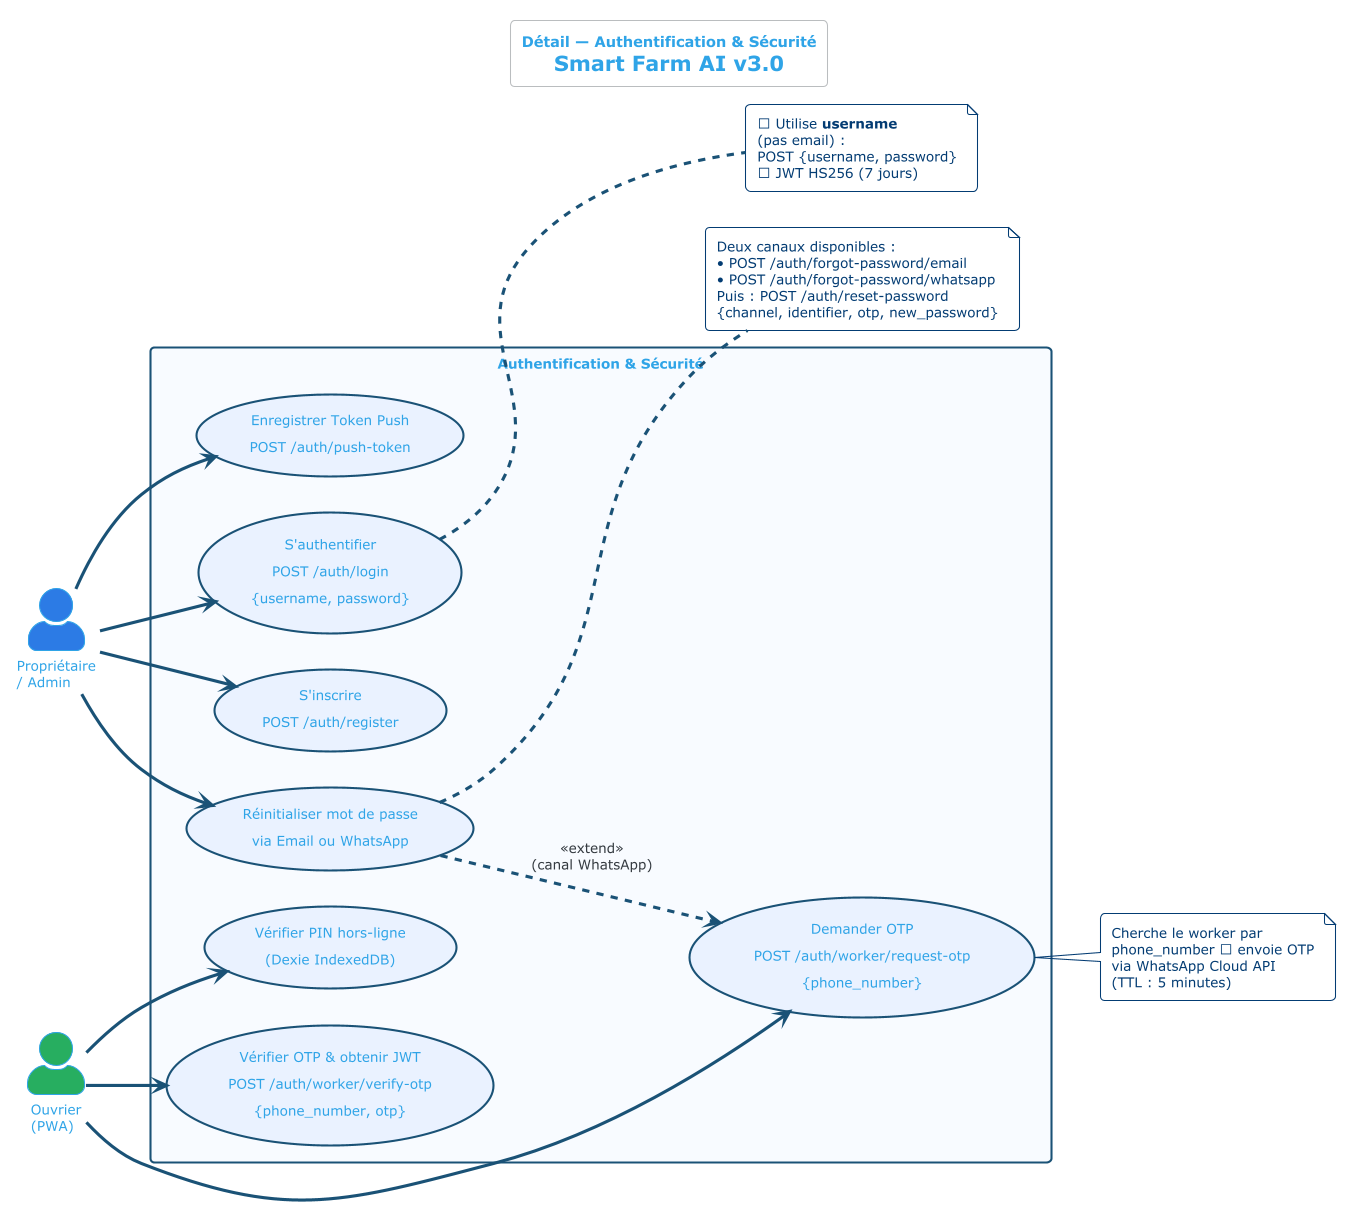
\includegraphics[width=0.95\textwidth]{figures/UC_Detail_Auth.png}
\caption[UC Authentification]{Diagramme UC détaillé --- Module Authentification et Sécurité.}
\label{fig:uc_auth}
\end{figure}

\paragraph{Module Authentification et Sécurité.}
La figure~\ref{fig:uc_auth} décrit les deux mécanismes d'accès du projet, fondés sur
les acteurs \textbf{admin owner} et \textbf{worker}. Le Propriétaire
s'authentifie par email et mot de passe, puis reçoit un token JWT HS256. L'Ouvrier
utilise un flux PIN puis OTP WhatsApp. Le contrôle RBAC est inclus dans chaque accès
aux ressources protégées afin de distinguer les rôles \texttt{owner} et
\texttt{worker}.

\begin{figure}[H]
\centering
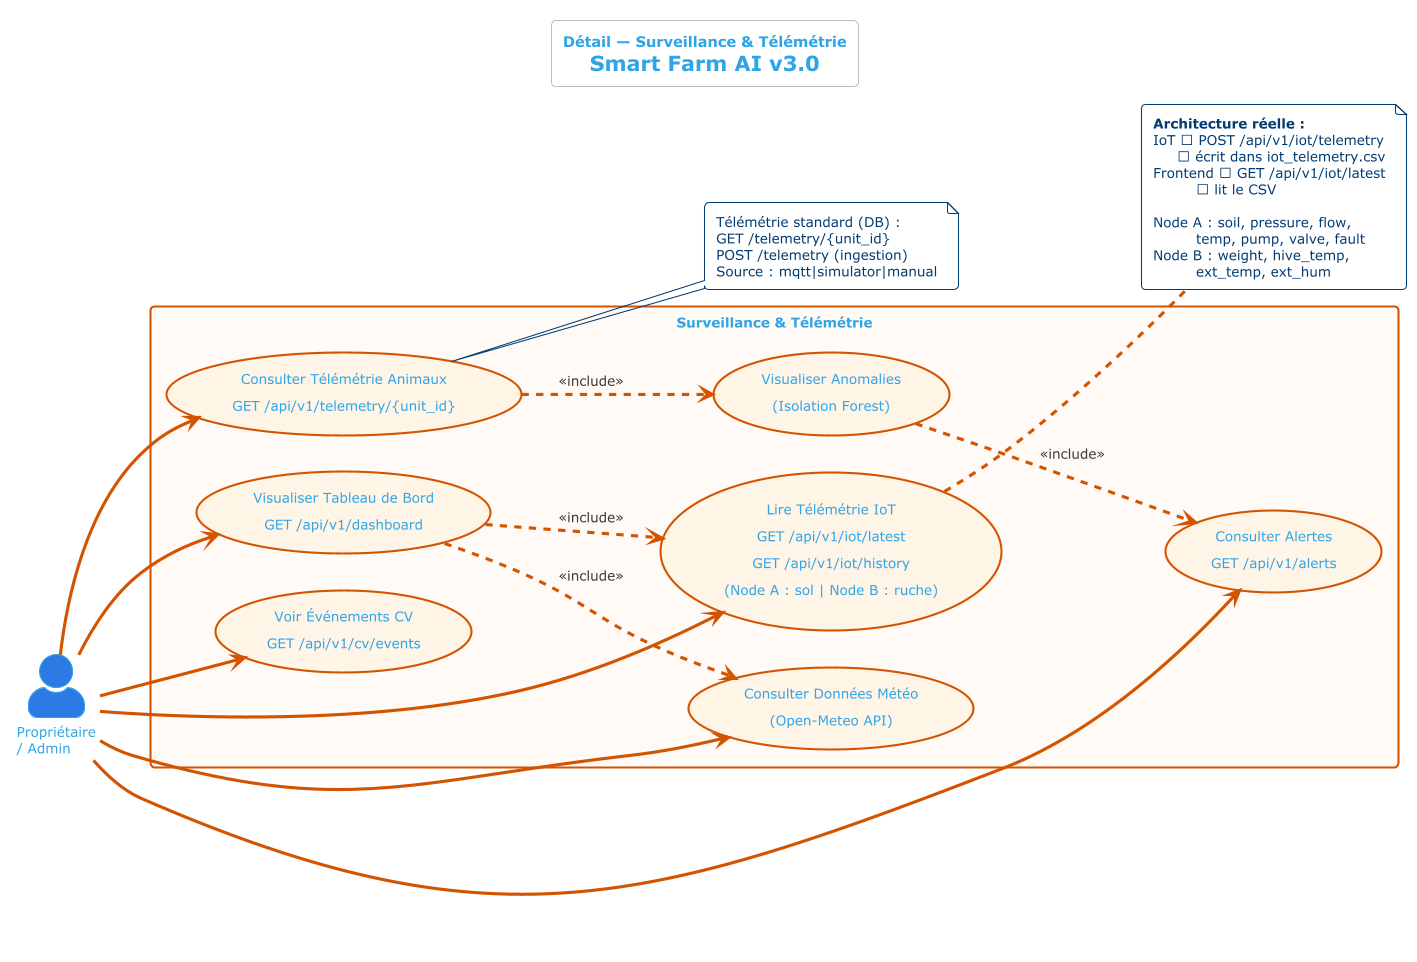
\includegraphics[width=0.95\textwidth]{figures/UC_Detail_Surveillance.png}
\caption[UC Surveillance IoT]{Diagramme UC détaillé --- Module Surveillance et Télémétrie IoT.}
\label{fig:uc_surveillance}
\end{figure}

\paragraph{Module Surveillance et Télémétrie IoT.}
La figure~\ref{fig:uc_surveillance} présente la consultation des données issues des
nœuds ESP32, l'historique des mesures et l'activation des actionneurs. Le cas
\textit{Générer alerte} étend la consultation de télémétrie lorsqu'un seuil critique
est dépassé, puis diffuse l'alerte par WebSocket multi-tenant.

\begin{figure}[H]
\centering
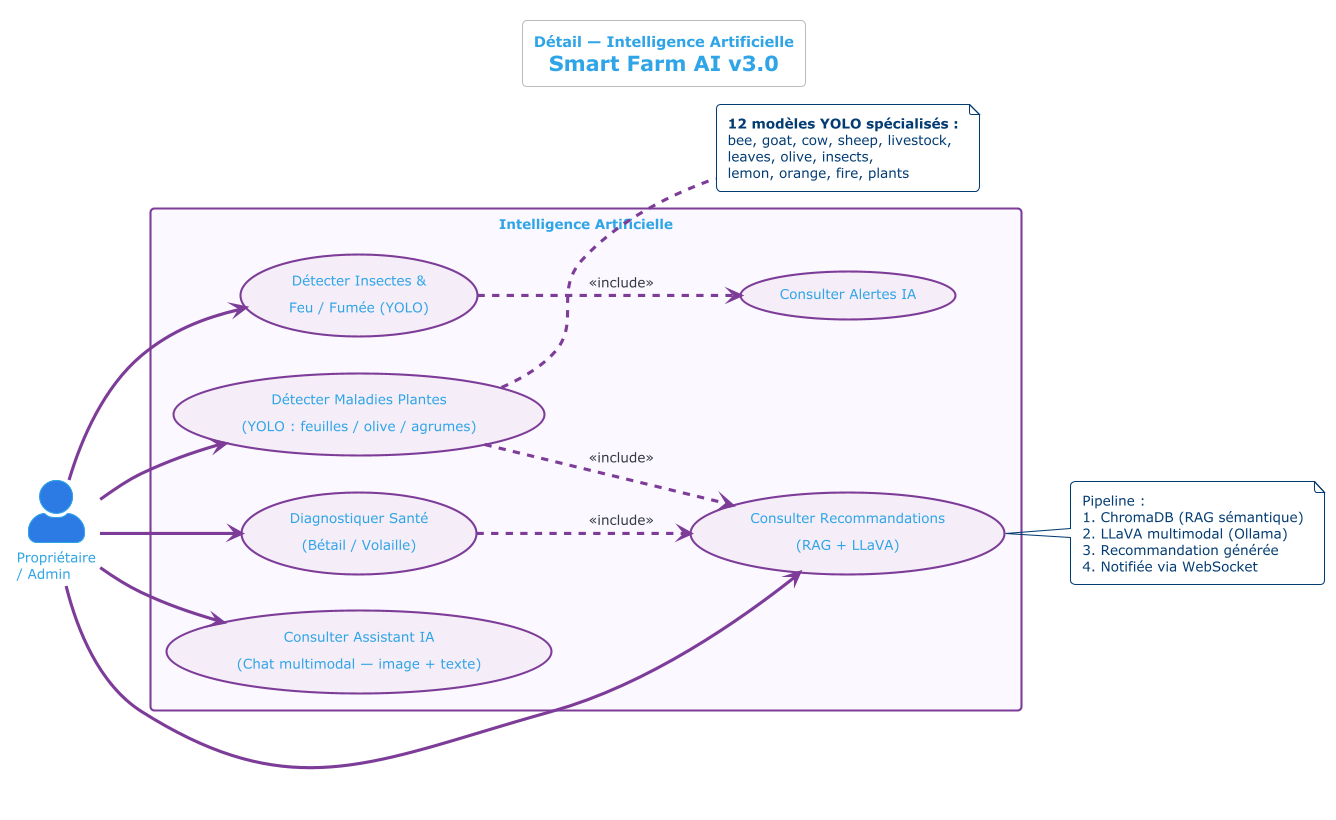
\includegraphics[width=0.95\textwidth]{figures/UC_Detail_IA.png}
\caption[UC Intelligence artificielle]{Diagramme UC détaillé --- Module Intelligence Artificielle.}
\label{fig:uc_ia}
\end{figure}

\paragraph{Module Intelligence Artificielle.}
La figure~\ref{fig:uc_ia} regroupe la détection visuelle et l'assistant Darija. Le
Propriétaire soumet une image au service YOLOv11, qui retourne la classe détectée, le
score de confiance et la boîte englobante. En parallèle, l'agent RAG récupère les
passages pertinents dans ChromaDB et génère une réponse en dialecte tunisien via
Ollama.

\begin{figure}[H]
\centering
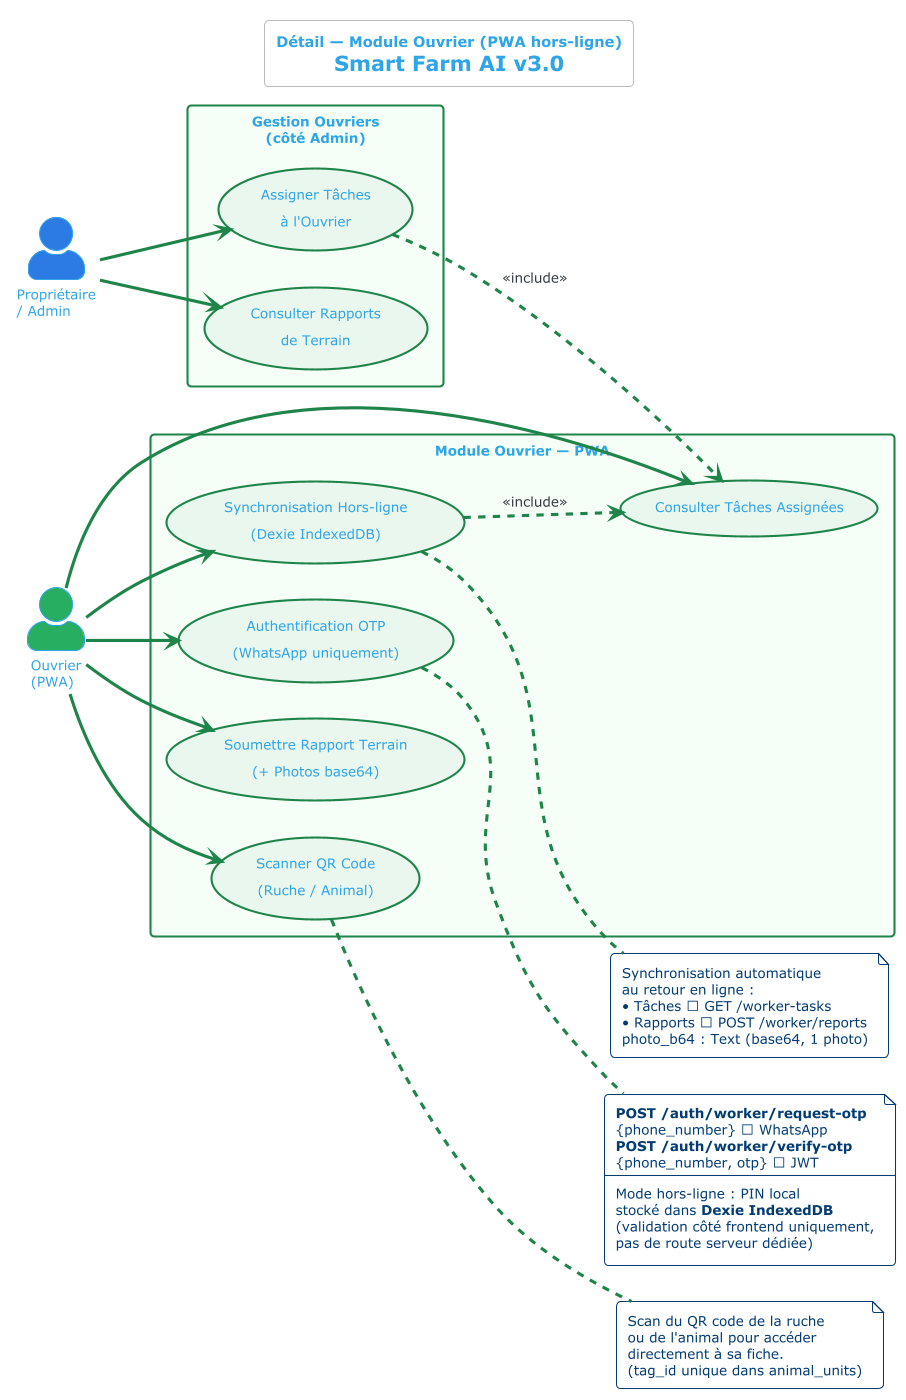
\includegraphics[width=0.95\textwidth]{figures/UC_Detail_Ouvrier.png}
\caption[UC Ouvrier PWA]{Diagramme UC détaillé --- Module Ouvrier PWA Offline.}
\label{fig:uc_ouvrier}
\end{figure}

\paragraph{Module Ouvrier PWA Offline.}
La figure~\ref{fig:uc_ouvrier} décrit les interactions mobiles de l'ouvrier :
validation des tâches, rapports terrain, photos, signalement sanitaire et consultation
des fiches de soin. Les actions réalisées hors-ligne sont stockées dans IndexedDB
puis synchronisées avec FastAPI dès le retour de la connexion.

\begin{figure}[H]
\centering
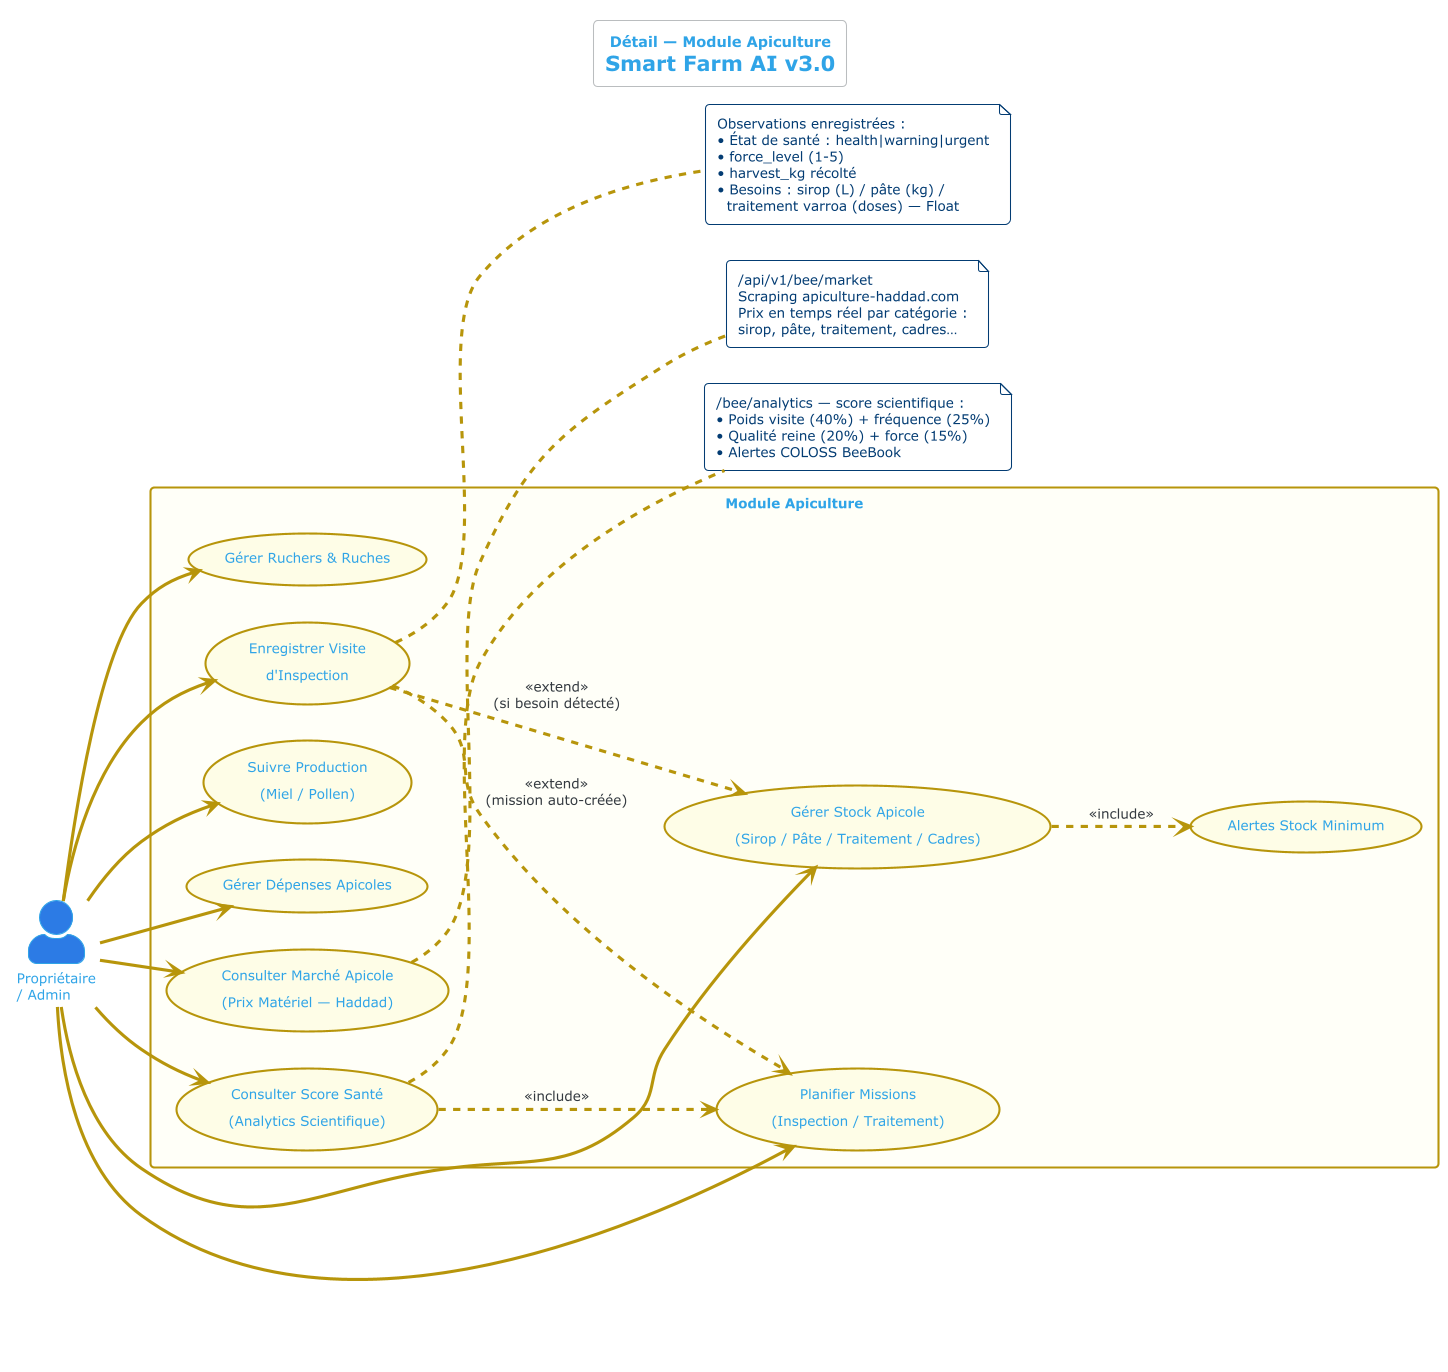
\includegraphics[width=0.95\textwidth]{figures/UC_Detail_Bee.png}
\caption[UC Apiculture]{Diagramme UC détaillé --- Module Apiculture.}
\label{fig:uc_bee}
\end{figure}

\paragraph{Module Apiculture.}
La figure~\ref{fig:uc_bee} couvre la gestion des ruchers, des ruches, des visites
COLOSS, des productions, des stocks et des dépenses. Les alertes d'essaimage ou de
température de couvain sont modélisées comme extensions conditionnelles du tableau de
bord IoT ruche.

\begin{figure}[H]
\centering
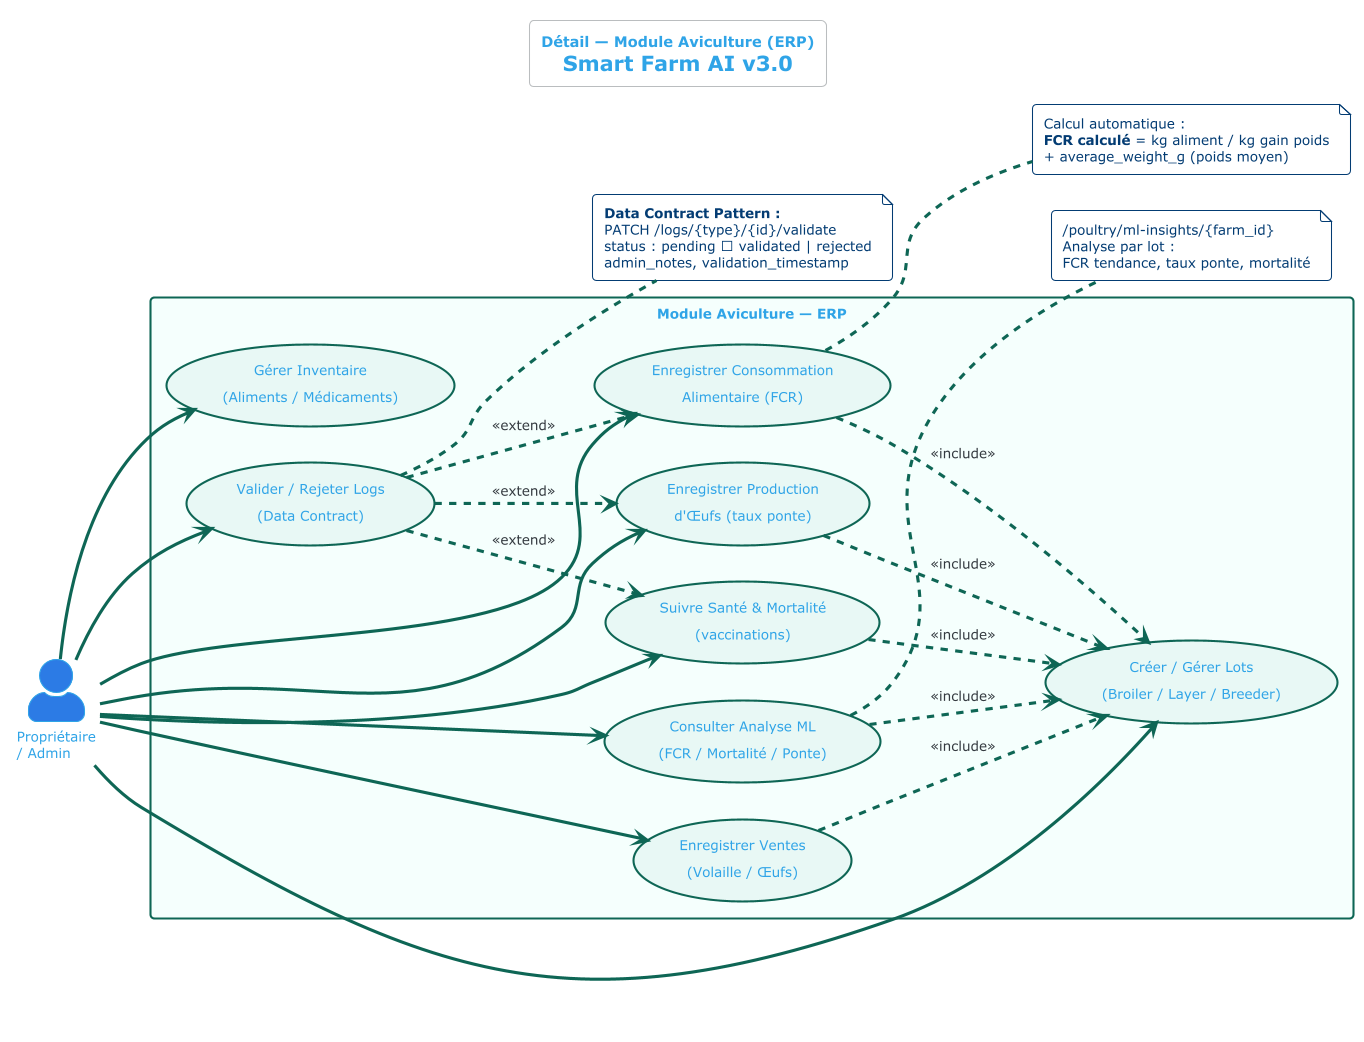
\includegraphics[width=0.95\textwidth]{figures/UC_Detail_Poultry.png}
\caption[UC Aviculture ERP]{Diagramme UC détaillé --- Module Aviculture ERP.}
\label{fig:uc_poultry}
\end{figure}

\paragraph{Module Aviculture ERP.}
La figure~\ref{fig:uc_poultry} formalise la gestion des lots avicoles, de
l'alimentation, de la mortalité, de la ponte, des soins, des ventes et des stocks.
Le cas \textit{Prédire FCR} est inclus dans le suivi du lot, tandis que la détection
d'anomalies et la comparaison aux standards de race sont des extensions du tableau de
bord.

% ── 2.2.4 Diagrammes de classes ──────────────────────────────
\subsection{Diagrammes de classes}
\label{sec:class}

Le modèle de classes de Smart Farm AI comprend \textbf{38 classes SQLAlchemy} et
six énumérations Python, réparties en sept packages fonctionnels. Les relations de
composition matérialisent les dépendances de cycle de vie, les associations représentent les liens
navigables et les dépendances indiquent les références facultatives entre entités.

\begin{figure}[H]
\centering
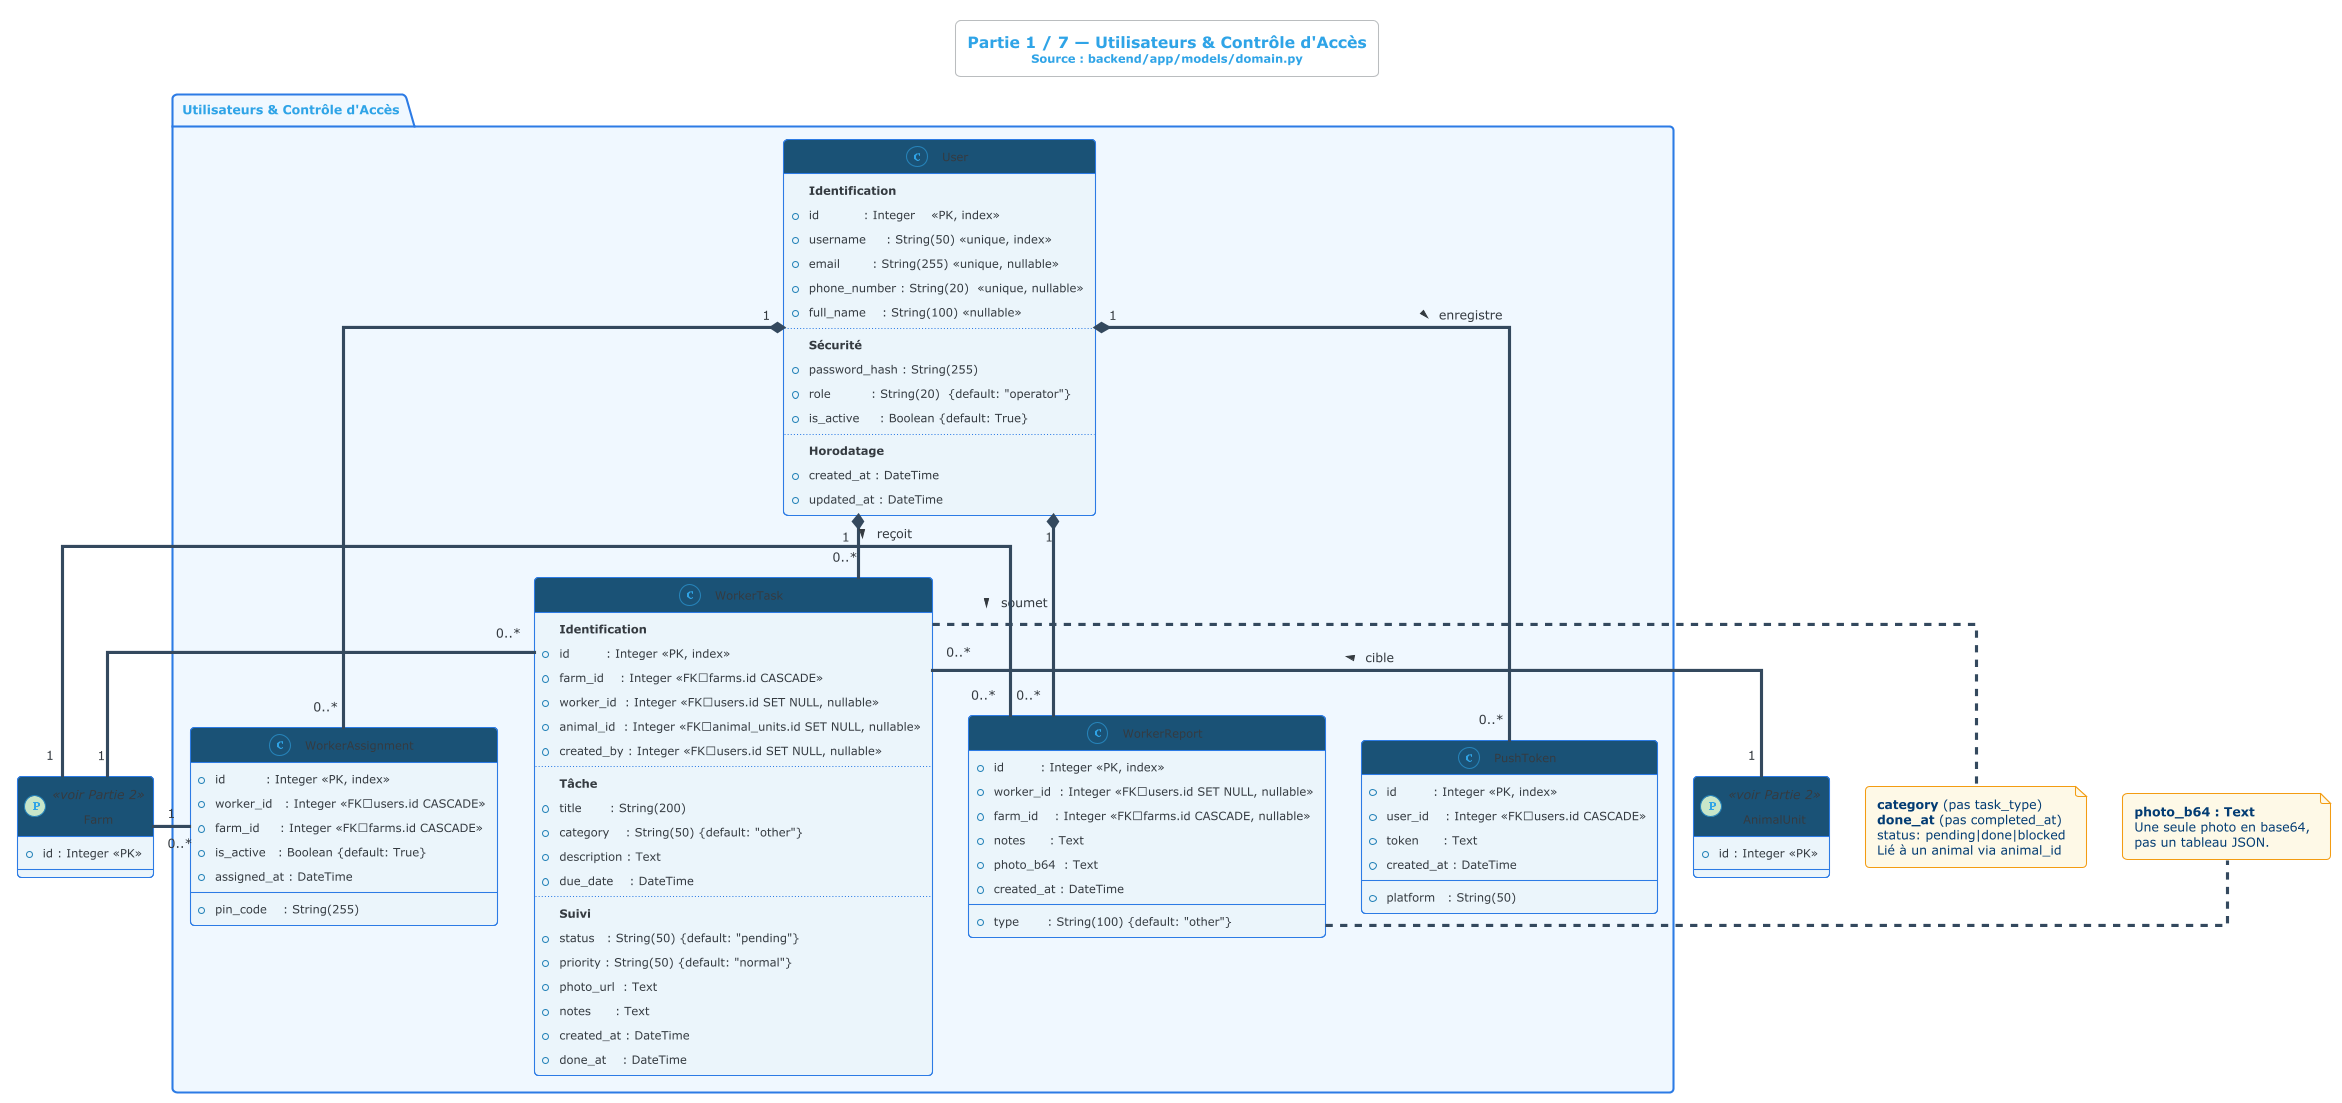
\includegraphics[width=0.95\textwidth]{figures/P1_Utilisateurs.png}
\caption[Classes P1 -- Utilisateurs]{Diagramme de classes --- package P1 : Utilisateurs et Accès.}
\label{fig:class_p1}
\end{figure}

\begin{figure}[H]
\centering
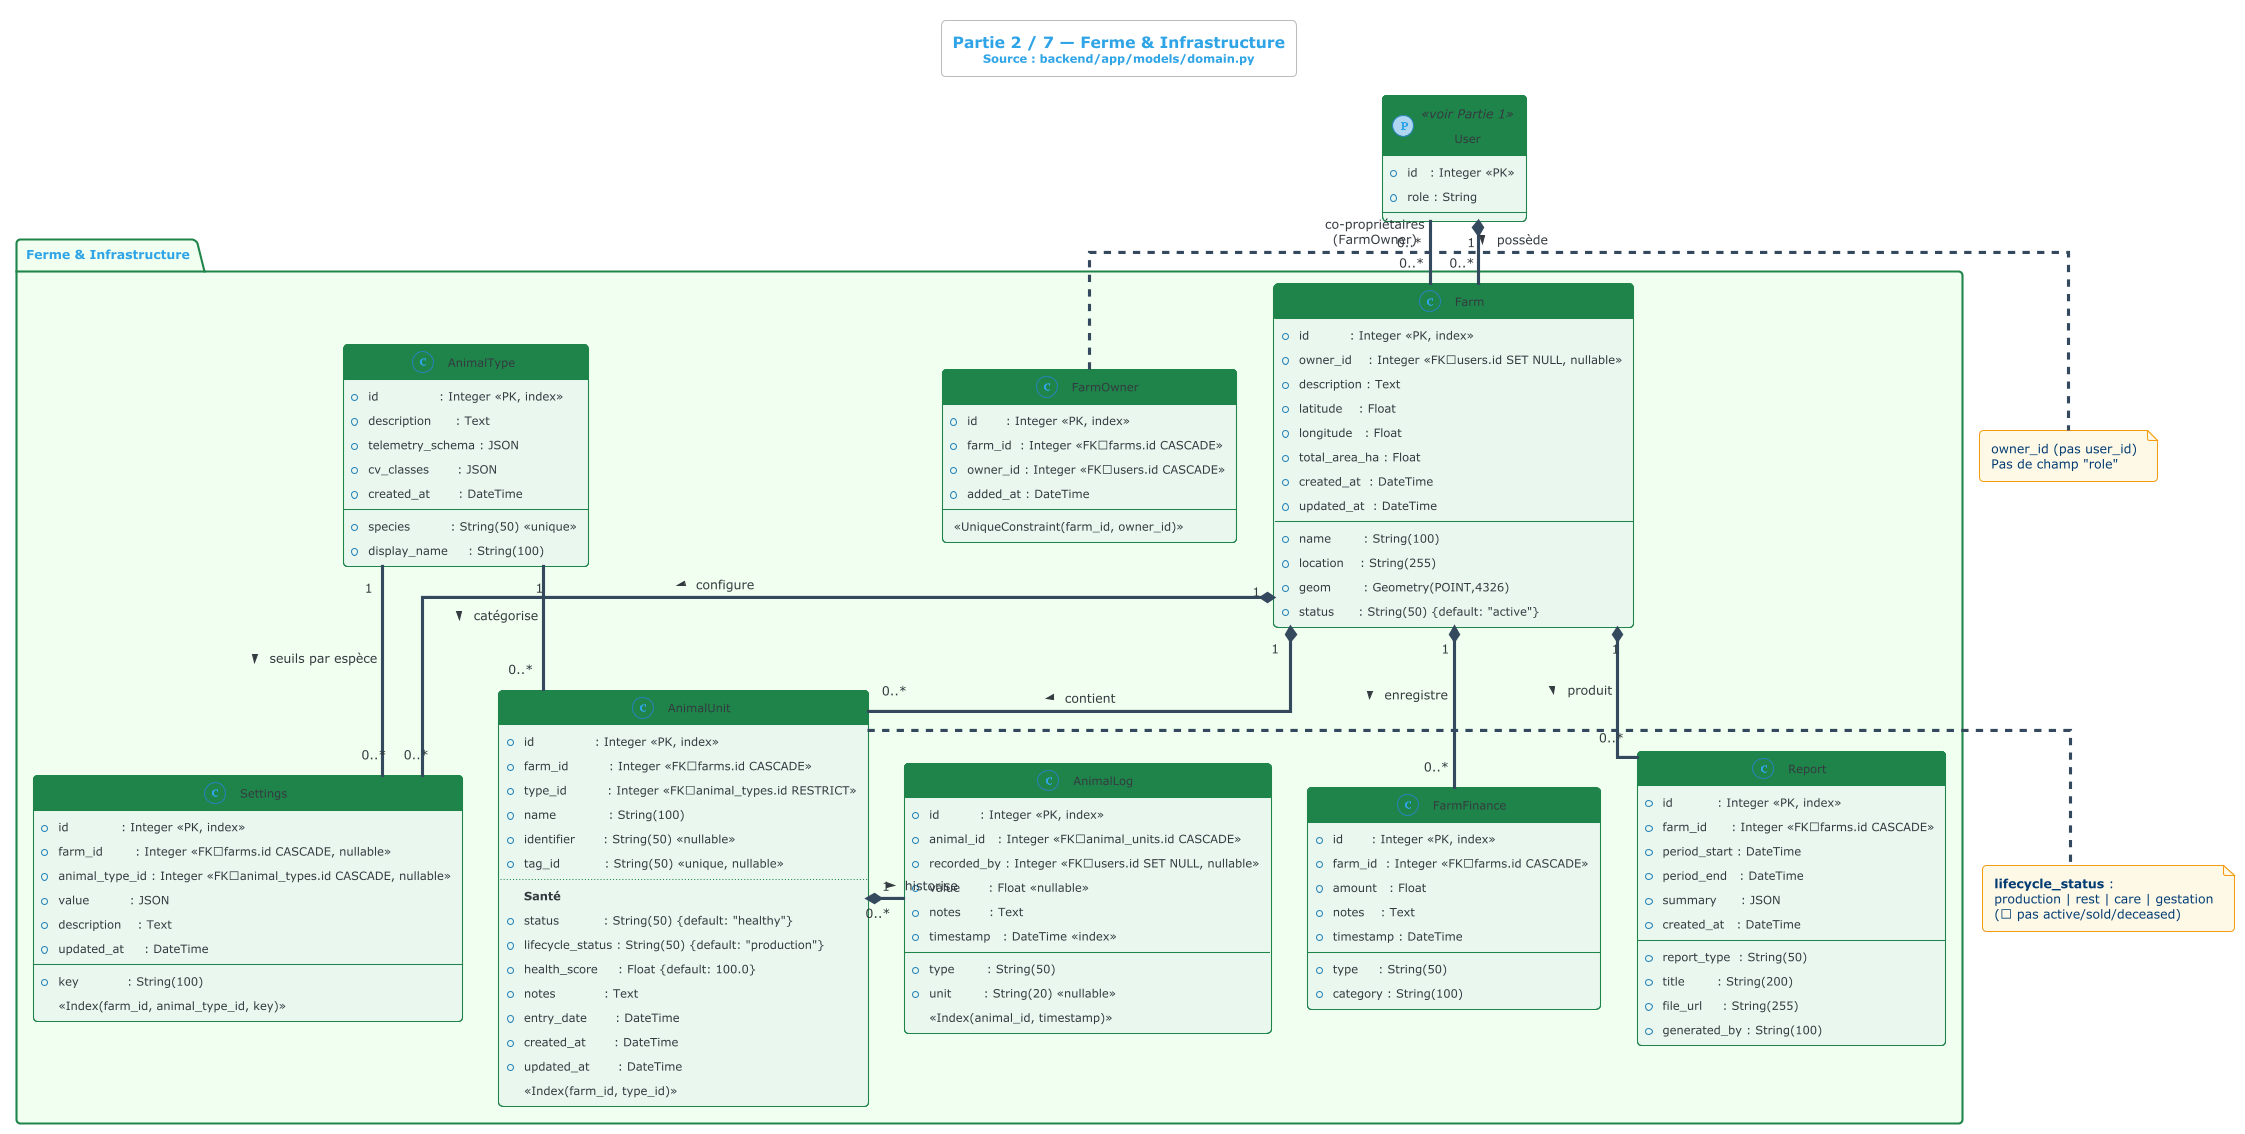
\includegraphics[width=0.95\textwidth]{figures/P2_Ferme_Infrastructure.png}
\caption[Classes P2 -- Ferme]{Diagramme de classes --- package P2 : Ferme et Infrastructure.}
\label{fig:class_p2}
\end{figure}

\paragraph{Packages P1 et P2.}
Le package P1 modélise les identités, les rôles et les affectations : \texttt{User},
\texttt{Owner}, \texttt{Worker}, \texttt{FarmOwner} et \texttt{WorkerAssignment}.
Le package P2 décrit la structure physique de l'exploitation à partir de
\texttt{Farm}, \texttt{AnimalUnit} et \texttt{Sensor}, avec les informations de
localisation, de statut et de cycle de vie des unités animales.

\begin{figure}[H]
\centering
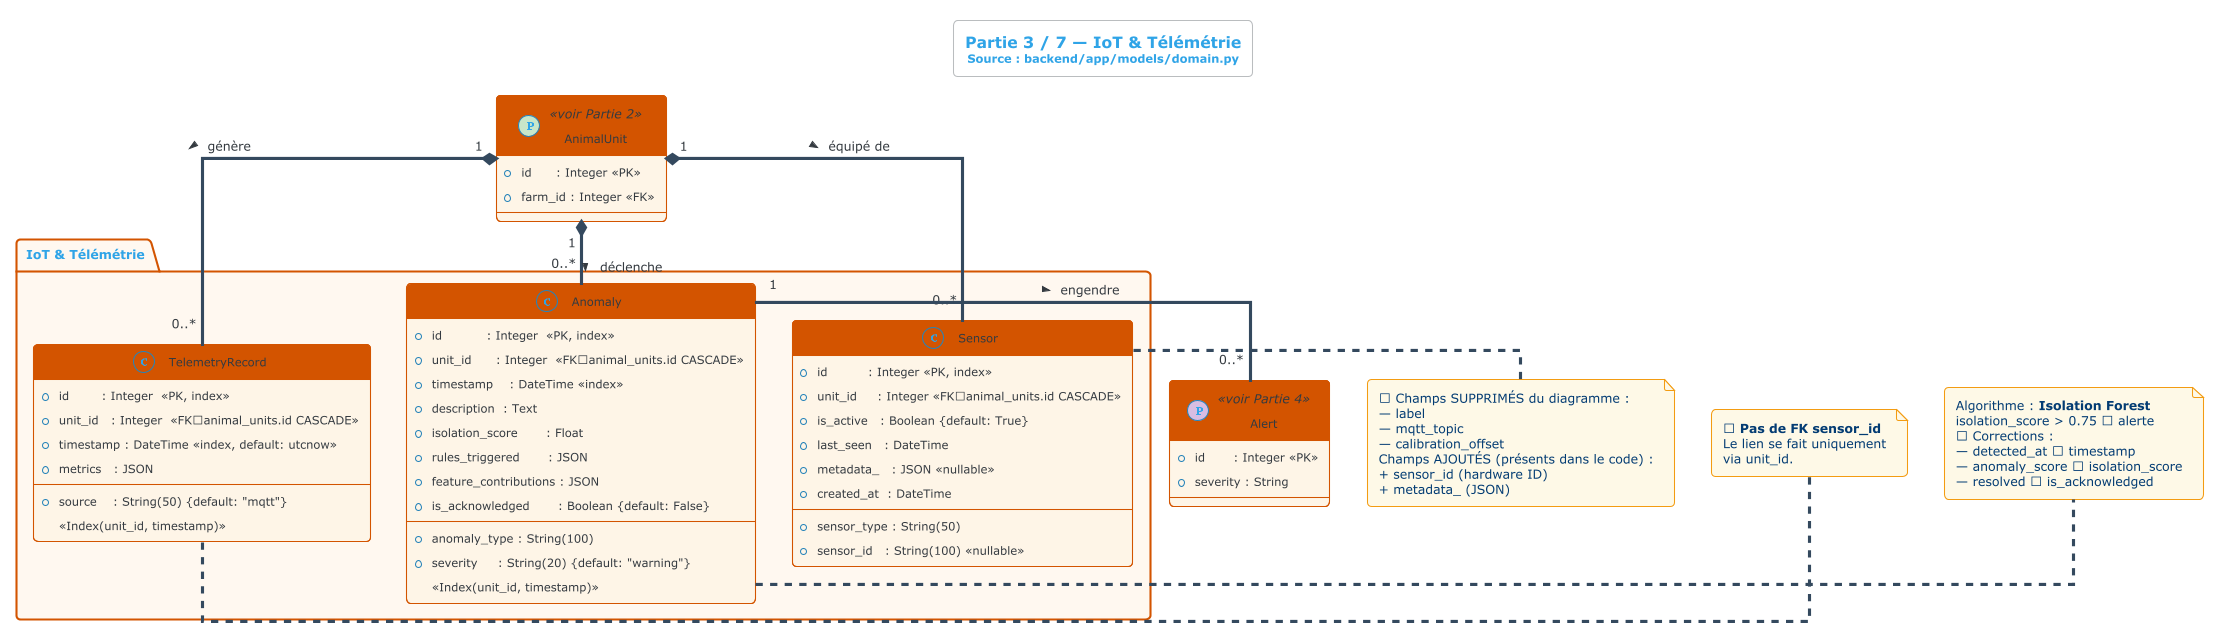
\includegraphics[width=0.95\textwidth]{figures/P3_IoT_Telemetrie.png}
\caption[Classes P3 -- IoT]{Diagramme de classes --- package P3 : IoT et Télémétrie.}
\label{fig:class_p3}
\end{figure}

\begin{figure}[H]
\centering
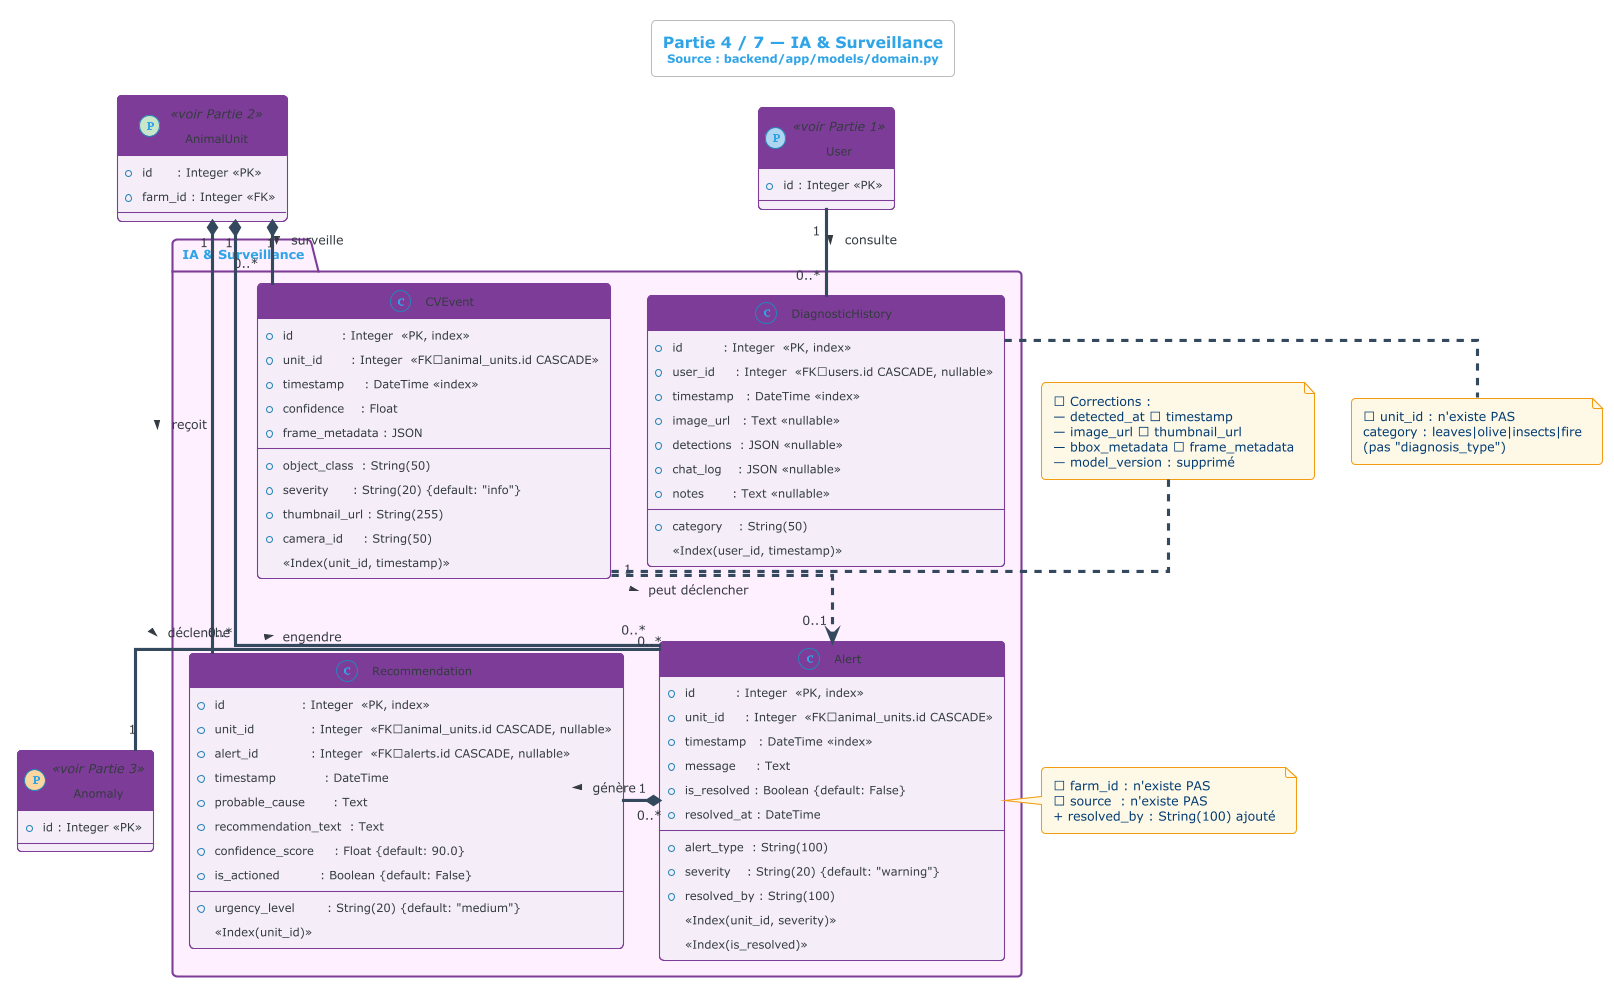
\includegraphics[width=0.95\textwidth]{figures/P4_IA_Surveillance.png}
\caption[Classes P4 -- IA]{Diagramme de classes --- package P4 : IA et Surveillance.}
\label{fig:class_p4}
\end{figure}

\paragraph{Packages P3 et P4.}
Le package P3 gère les mesures \texttt{TelemetryRecord}, les anomalies, les alertes
et les paramètres de seuils. Le package P4 archive les événements de vision par
ordinateur avec \texttt{CVEvent}, les recommandations RAG avec \texttt{Recommendation}
et l'historique des diagnostics dans \texttt{DiagnosticHistory}.

\begin{figure}[H]
\centering
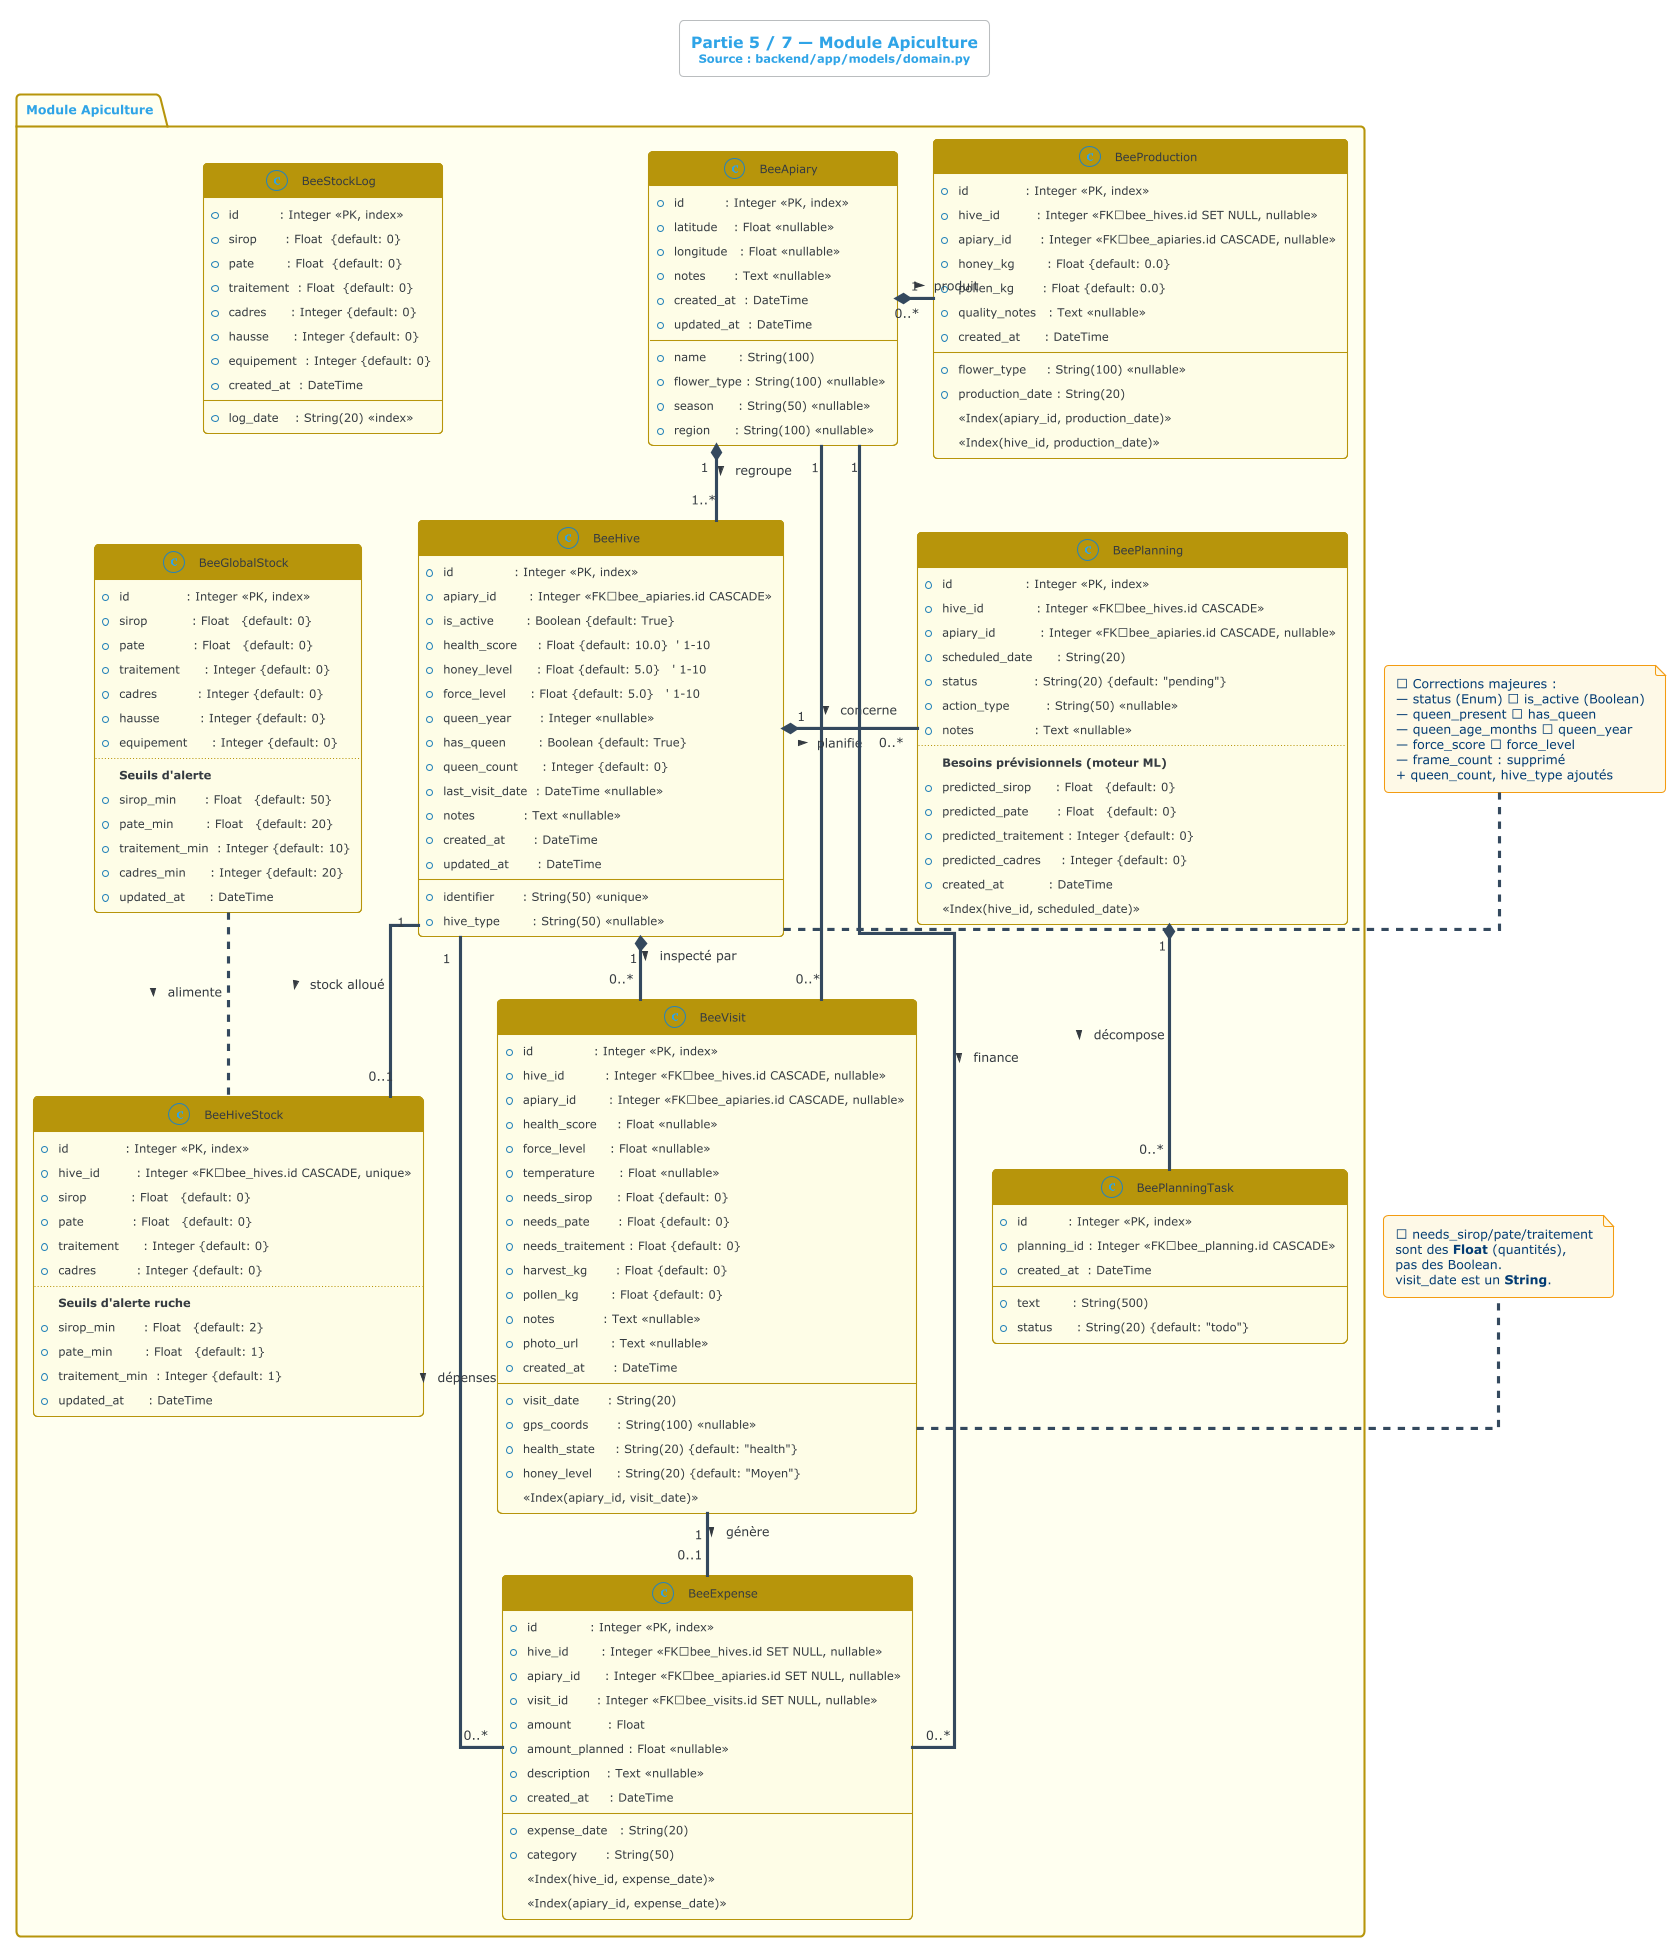
\includegraphics[width=0.95\textwidth]{figures/P5_Apiculture.png}
\caption[Classes P5 -- Apiculture]{Diagramme de classes --- package P5 : Apiculture.}
\label{fig:class_p5}
\end{figure}

\begin{figure}[H]
\centering
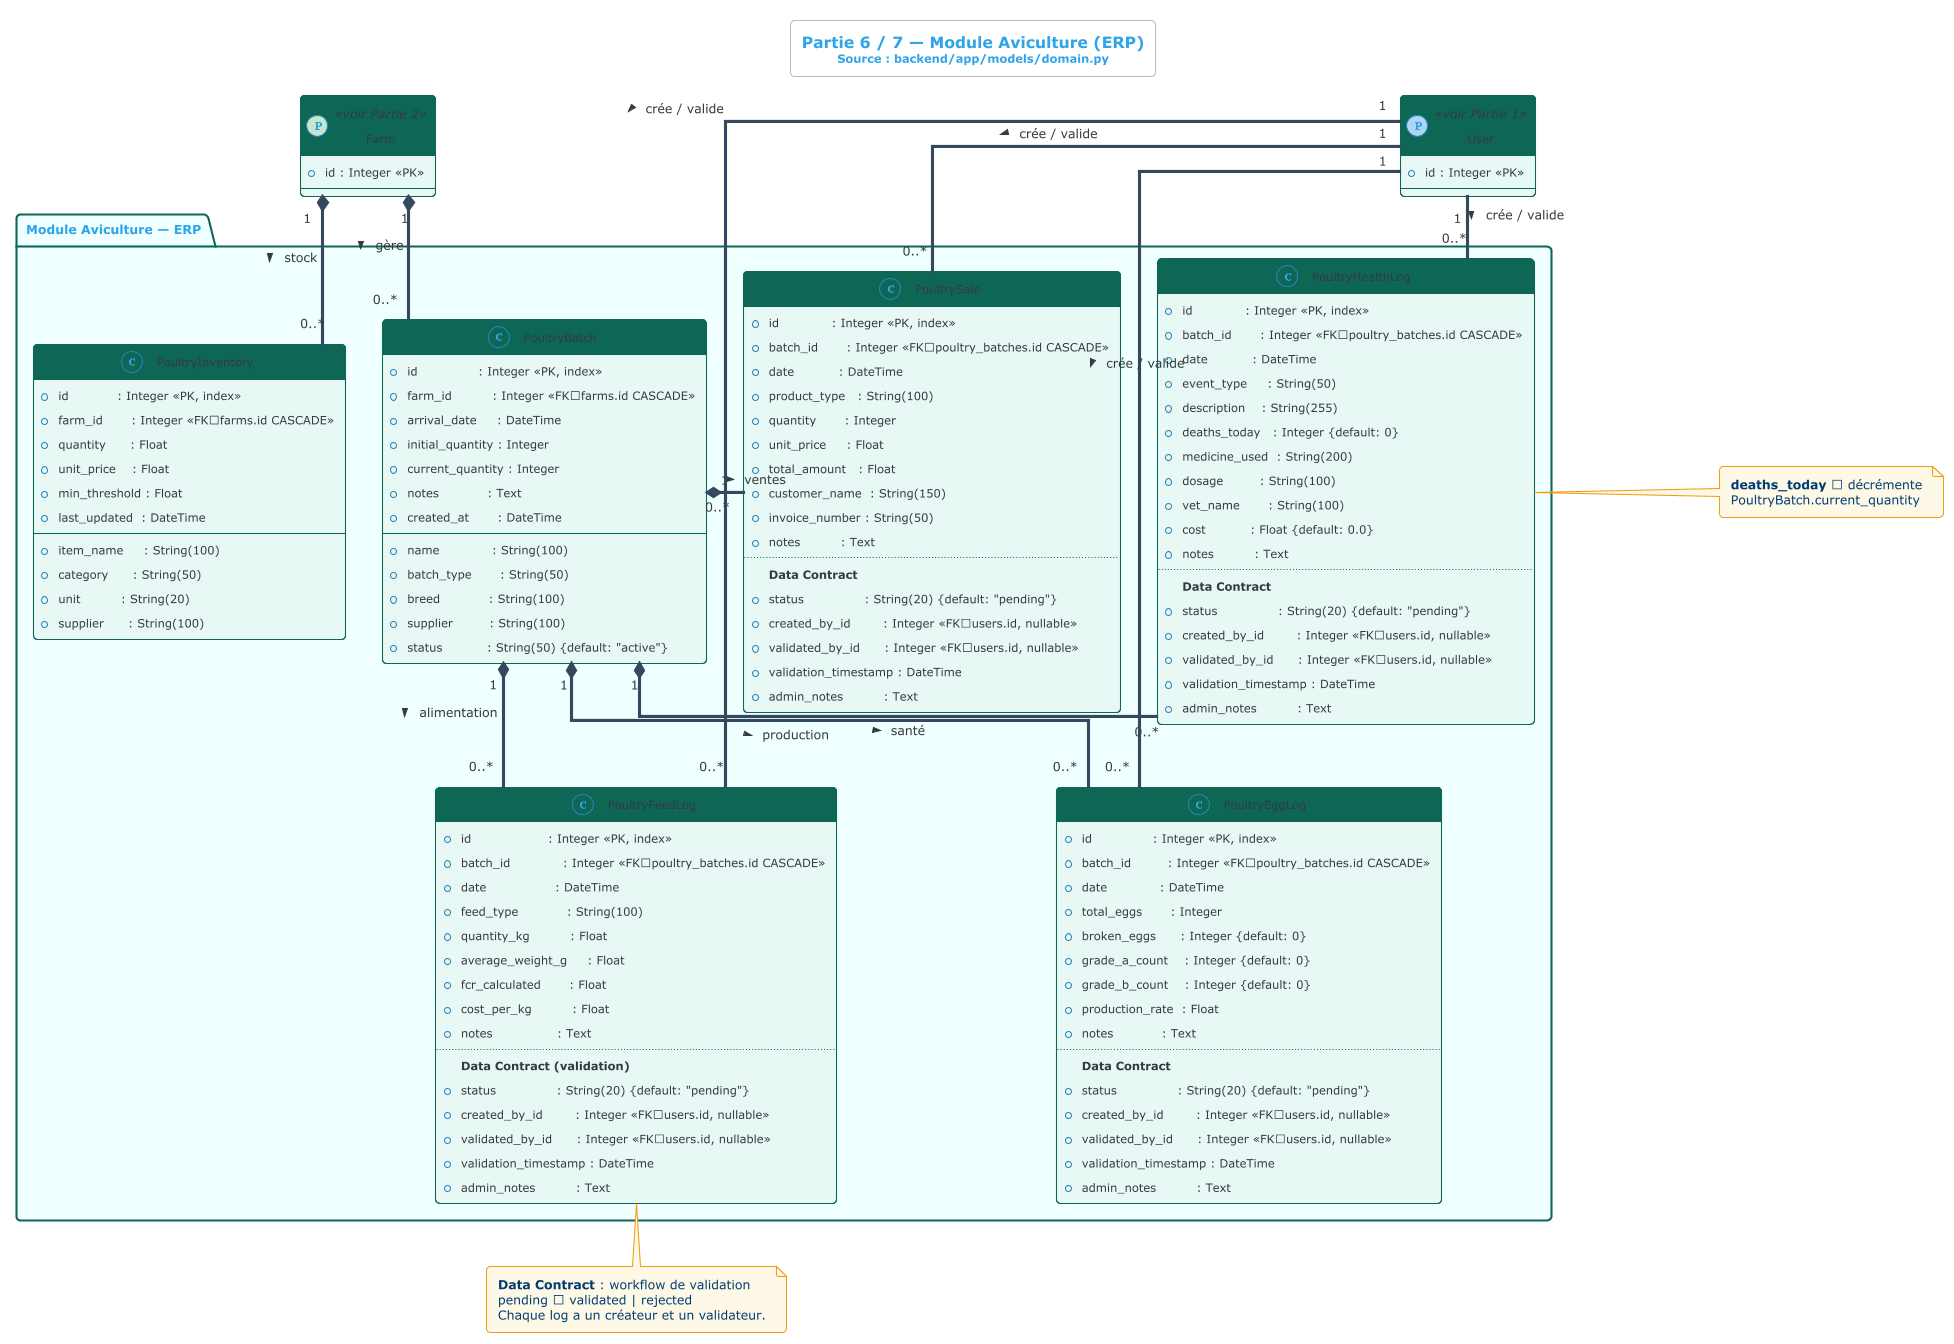
\includegraphics[width=0.95\textwidth]{figures/P6_Aviculture_ERP.png}
\caption[Classes P6 -- Aviculture]{Diagramme de classes --- package P6 : Aviculture ERP.}
\label{fig:class_p6}
\end{figure}

\paragraph{Packages P5 et P6.}
Le package P5 couvre le cycle apicole complet : ruchers, ruches, visites COLOSS,
productions, stocks, dépenses et planification. Le package P6 implémente l'ERP
avicole autour de \texttt{PoultryBatch}, avec les enregistrements d'alimentation,
de mortalité, de ponte, de santé et de ventes.

\begin{figure}[H]
\centering
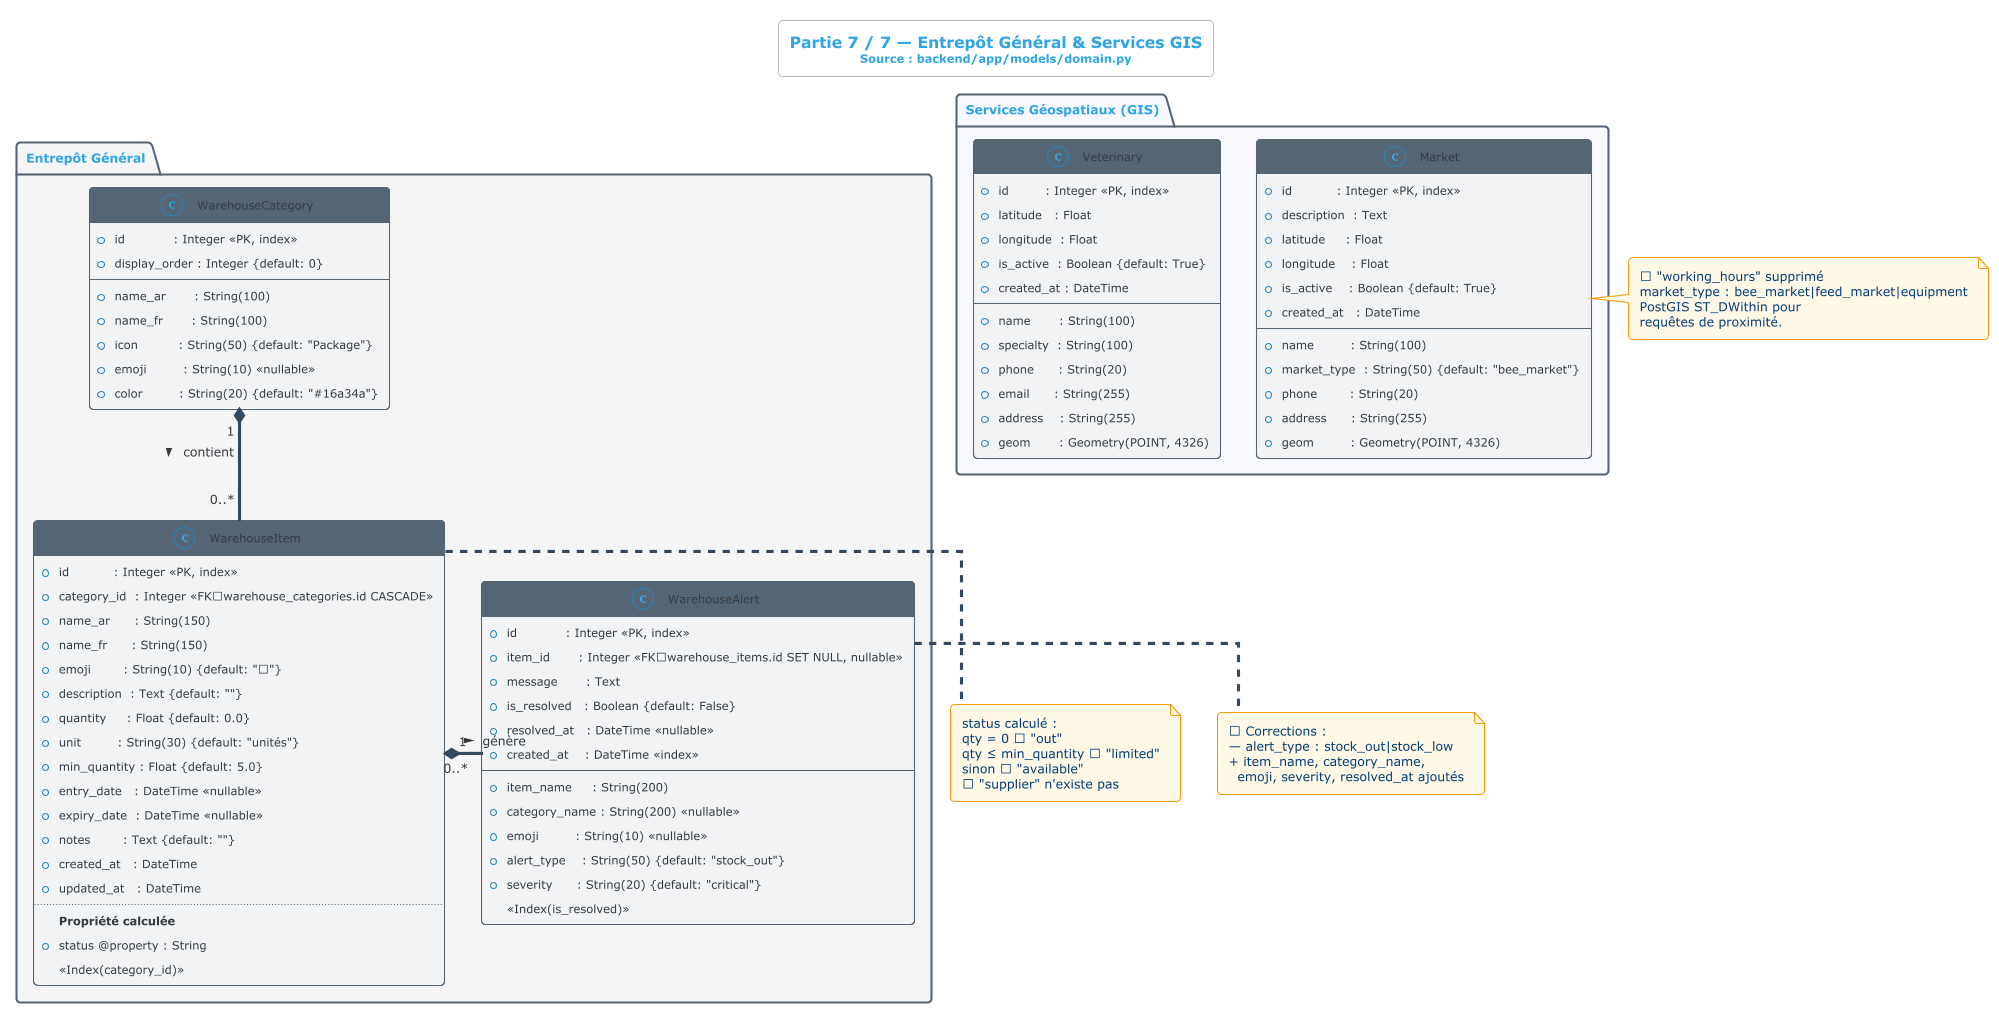
\includegraphics[width=0.95\textwidth]{figures/P7_Entrepot_GIS.png}
\caption[Classes Entrepôt et GIS]{Diagramme de classes --- package Entrepôt et GIS.}
\label{fig:class_p7}
\end{figure}

\paragraph{Package P7 --- Entrepôt et GIS.}
La figure~\ref{fig:class_p7} regroupe les entités géospatiales exploitées par le
module cartographique, notamment les vétérinaires et les marchés agricoles. Les
recherches de proximité s'appuient sur PostGIS en mode PostgreSQL et sur la formule
de Haversine en mode léger SQLite.

% ── 2.3 Revue des travaux récents ───────────────────────────
\section{Revue des travaux récents}

Cette section analyse six contributions scientifiques récentes couvrant les domaines
technologiques fondateurs du projet : IoT agricole, vision par ordinateur,
prédiction avicole, génération augmentée par récupération (RAG) et modèles de
langage souverains. Pour chaque article, nous présentons les apports principaux
et les limites qui ont orienté nos choix de conception.

\subsection*{Article 1 --- Smart Farming et IoT multi-nœuds}

Sharma \textit{et al.}~\cite{sharma2024smart} proposent un système IoT multi-nœuds
pour l'agriculture de précision intégrant des capteurs environnementaux (température,
humidité, conductivité du sol) et des actionneurs connectés via MQTT.
Leur architecture centralisée sur serveur cloud permet la supervision en temps réel
de parcelles distribuées et l'activation automatique de l'irrigation selon des
seuils configurables. Les auteurs reportent une réduction de $23\,\%$ de la
consommation d'eau et une amélioration du rendement de $17\,\%$ sur des exploitations
céréalières de la région MENA.
Cette architecture MQTT multi-nœuds constitue le modèle direct de notre sous-système
IoT avec deux nœuds ESP32 dédiés à l'irrigation et au monitoring de ruche.

\subsection*{Article 2 --- Deep Learning en agriculture}

Kamilaris et Prenafeta-Boldú~\cite{kamilaris2018} ont conduit une revue systématique
de 40 études appliquant le deep learning à l'agriculture.
Ils concluent que les réseaux convolutifs (CNN) surpassent les méthodes classiques
de $+15$ à $+25$ points de précision pour la classification des maladies foliaires
et la détection d'insectes ravageurs.
Leurs résultats démontrent la supériorité du transfer learning (ImageNet $\rightarrow$
domaine agricole) lorsque les jeux de données annotés sont de taille limitée,
ce qui justifie notre stratégie de fine-tuning YOLOv11 sur des datasets agricoles
tunisiens.

\subsection*{Article 3 --- YOLO pour la détection de bétail}

Chen \textit{et al.}~\cite{chen2023yolo_livestock} ont comparé cinq variantes YOLO
(v5s, v7, v8n, v8s, v8m) pour la détection et le comptage de bétail en feedlot.
YOLOv11n offre le meilleur compromis vitesse/précision avec une inférence
$\leq 200$\,ms sur CPU embarqué et un mAP@50 de $91.3\,\%$ sur leur jeu de test.
Ils soulignent que l'architecture \textit{anchor-free} à têtes découplées de YOLOv11
améliore significativement le rappel sur les petits objets.
Notre déploiement sur serveur agricole à ressources limitées reproduit ce choix
architectural et étend la détection à 11 classes (bovins, ovins, caprins,
abeilles, pathologies foliaires, feux\ldots).

\subsection*{Article 4 --- Prédiction du FCR en aviculture}

Zhang \textit{et al.}~\cite{zhang2023fcr} ont modélisé le taux de conversion
alimentaire (FCR) de poulets de chair par régression polynomiale et réseaux LSTM
sur un corpus de 1\,200 lots, obtenant $R^2 \in [0.87, 0.93]$.
Ils démontrent que la régression polynomiale de degré~2 est particulièrement adaptée
à la dynamique de croissance avicole sur la fenêtre 7--42 jours (courbe sigmoïdale
linéarisable), tout en offrant une interprétabilité supérieure aux réseaux LSTM
pour les éleveurs.
Notre approche polynomiale ($R^2 = 0.891 \pm 0.024$) confirme ce résultat de
référence et valide le choix d'un modèle interprétable plutôt qu'une boîte noire.

\subsection*{Article 5 --- Génération augmentée par récupération (RAG)}

Lewis \textit{et al.}~\cite{lewis2020rag} ont introduit le paradigme RAG
(\textit{Retrieval-Augmented Generation}) comme alternative à la mémorisation
paramétrique dans les LLM. En combinant un encodeur de récupération dense (DPR)
et un générateur seq2seq (BART), ils obtiennent $\text{EM} = 44.5\,\%$
sur NaturalQuestions, surpassant les modèles purement paramétriques.
Ce paradigme est fondamental dans notre architecture~: l'assistant Darija
récupère dynamiquement des passages pertinents des guides AVFA et des fiches
vétérinaires tunisiennes stockés dans ChromaDB avant de générer sa réponse.

\subsection*{Article 6 --- RAG pour la recommandation agricole}

Zheng \textit{et al.}~\cite{zheng2024rag_agri} ont appliqué RAG à la recommandation
agricole (gestion des sols, sélection de cultures) en combinant des corpus en anglais
et mandarin, rapportant une amélioration de $+18\,\%$ du BLEU-4 par rapport à un
LLM seul. Leur architecture (ChromaDB + GPT-3.5, chunking 512 tokens) constitue
le modèle direct de notre pipeline RAG.
Notre contribution étend cette approche au dialecte tunisien Darija, une langue
à très faibles ressources NLP~\cite{abbou2024arabic}, en intégrant des corpus
agronomiques locaux (BLEU-4~$= 0.68$, Cohen's $\kappa = 0.76$).

\subsection{Tableau comparatif des articles}

Le tableau~\ref{tab:comparatif_articles} synthétise et compare les caractéristiques
techniques des six articles analysés, puis positionne Smart Farm AI au regard de
chacune de ces contributions.

\begin{table}[H]
\centering
\caption[Travaux récents en agriculture]{Tableau comparatif des travaux récents en agriculture intelligente}
\label{tab:comparatif_articles}
\resizebox{\textwidth}{!}{%
\tiny\setlength{\tabcolsep}{2pt}%
\begin{tabular}{>{\RaggedRight\arraybackslash}p{2.2cm}>{\RaggedRight\arraybackslash}p{2.8cm}>{\RaggedRight\arraybackslash}p{2.4cm}>{\RaggedRight\arraybackslash}p{1.8cm}>{\RaggedRight\arraybackslash}p{2.6cm}>{\RaggedRight\arraybackslash}p{2.5cm}
                >{\RaggedRight\arraybackslash}p{2.2cm}>{\RaggedRight\arraybackslash}p{2.2cm}>{\RaggedRight\arraybackslash}p{2.4cm}>{\RaggedRight\arraybackslash}p{2.4cm}>{\RaggedRight\arraybackslash}p{2.6cm}>{\RaggedRight\arraybackslash}p{2.4cm}}
\toprule
\textbf{Source \& Année} &
\textbf{Objectif principal} &
\textbf{Méthode / Modèle} &
\textbf{Type de tâche} &
\textbf{Backbone / Architecture} &
\textbf{Techniques clés} &
\textbf{Jeux de données} &
\textbf{Performance} &
\textbf{Avantages} &
\textbf{Limites} &
\textbf{Contributions clés} &
\textbf{Perspectives futures} \\
\midrule

Sharma \textit{et al.}~\cite{sharma2024smart}\,(2024) &
Supervision IoT multi-nœuds agriculture de précision &
Architecture MQTT centralisée, capteurs env. &
Monitoring, automatisation &
ESP32, broker MQTT, cloud &
QoS~1, capteurs sol/air, actionneurs &
Parcelles MENA &
$-23\,\%$ eau, $+17\,\%$ rendement &
Multi-nœuds, faible latence réseau rural &
Dépendance cloud, sans ML prédictif &
Premier système IoT multi-nœuds MQTT MENA &
IA embarquée, Edge computing \\
\midrule

Kamilaris \& Prenafeta~\cite{kamilaris2018}\,(2018) &
Revue DL en agriculture (40 études) &
CNN : AlexNet, VGG, ResNet &
Classification, détection &
Réseaux CNN convolutifs &
Transfer learning, augmentation &
PlantVillage, insects &
$+15$--$25$ pts vs. classique &
Revue exhaustive, preuve CNN &
Dépendant des datasets &
Validation transfer learning agri. &
Datasets multilingues, ruraux \\
\midrule

Chen \textit{et al.}~\cite{chen2023yolo_livestock}\,(2023) &
Détection et comptage bétail en feedlot &
YOLOv11n vs. v5/v7 (5 variantes) &
Détection d'objets &
YOLOv11n anchor-free &
NMS, mosaic augmentation &
Feedlot 5\,000 frames &
mAP@50\,$=91.3\,\%$, $\leq200$\,ms CPU &
CPU embarqué, temps réel, open-source &
Espèce unique, sans pathologie &
Meilleur compromis YOLOv11n CPU &
Multi-espèces, pathologies \\
\midrule

Zhang \textit{et al.}~\cite{zhang2023fcr}\,(2023) &
Prédiction FCR poulets (1\,200 lots) &
Régression poly.~deg.~2 + LSTM~128 &
Régression supervisée &
Polynomial + LSTM, 5-fold CV &
Feature engineering, TimeSeriesSplit &
1\,200 lots avicoles &
$R^2 \in [0.87,\,0.93]$ &
Interprétabilité, performances sur 7--42j &
Pas de généralisation multi-race &
Premier modèle FCR polynomial Afrique Nord &
Multi-race, IoT temps réel \\
\midrule

Lewis \textit{et al.}~\cite{lewis2020rag}\,(2020) &
Génération augmentée par récupération (RAG) &
DPR + BART seq2seq &
QA ouvert, génération cond. &
BERT biencoder + BART &
Retrieval dense top-$k$ &
NaturalQuestions, TriviaQA &
EM\,$=44.5\,\%$ (NQ) &
Réductibilité mémoire, corpus flexible &
Latence retrieval, qualité corpus &
Introduction paradigme RAG &
RAG multilingue, corpus rares \\
\midrule

Zheng \textit{et al.}~\cite{zheng2024rag_agri}\,(2024) &
Recommandation agricole via RAG &
RAG + GPT-3.5, ChromaDB &
QA agricole, recommandation &
ChromaDB + GPT-3.5 &
Chunking 512 tok., top-$k=5$ &
Corpus sols/cultures CN+EN &
$+18\,\%$ BLEU-4 vs. LLM seul &
Corpus multilingue, spécialisé &
Langues africaines absentes &
Premier RAG agricole CN/EN évalué &
Dialectes arabes, Darija \\
\midrule

\textbf{Smart Farm AI} (ce travail) &
Plateforme intégrée multi-espèces IoT + YOLO + RAG Darija &
YOLOv11 + poly ML + RAG + Labess-7B &
Détection, régression, QA Darija, IoT &
FastAPI + YOLOv11 + ChromaDB + Ollama + ESP32 &
anchor-free, 5-fold CV, IC~95\,\% bootstrap, DVC &
11 classes YOLO, 500+ lots, 312 chunks AVFA &
mAP@50\,$=84.7\,\%$, $R^2=0.891$, BLEU-4\,$=0.68$ &
Multi-espèces, souverain, Darija, offline PWA &
Contexte tunisien, monodéploiement &
$1^\text{re}$ éval. quantitative Darija élevage &
Multi-pays, foundation models Maghreb \\

\bottomrule
\end{tabular}
}%
\end{table}

\medskip

L'analyse de ce tableau révèle que Smart Farm AI intègre et dépasse ces contributions
individuelles en combinant IoT multi-nœuds~\cite{sharma2024smart}, détection YOLO
multi-classes~\cite{chen2023yolo_livestock}, prédiction avicole~\cite{zhang2023fcr}
et RAG souverain en Darija~\cite{zheng2024rag_agri} au sein d'une architecture unifiée,
open-source et opérationnelle hors-ligne.

% ── 2.4 Architecture du projet ──────────────────────────────
\section{Architecture du projet}

L'architecture de Smart Farm AI a été conçue selon le principe de séparation des
responsabilités (\textit{Separation of Concerns}). Elle repose sur une structure
modulaire en quatre couches interdépendantes permettant l'évolutivité du système
et sa maintenance indépendante par module.
La figure~\ref{fig:archi_globale} présente la vue globale du système, depuis
les nœuds IoT terrain jusqu'aux interfaces utilisateurs.

\begin{figure}[H]
\centering
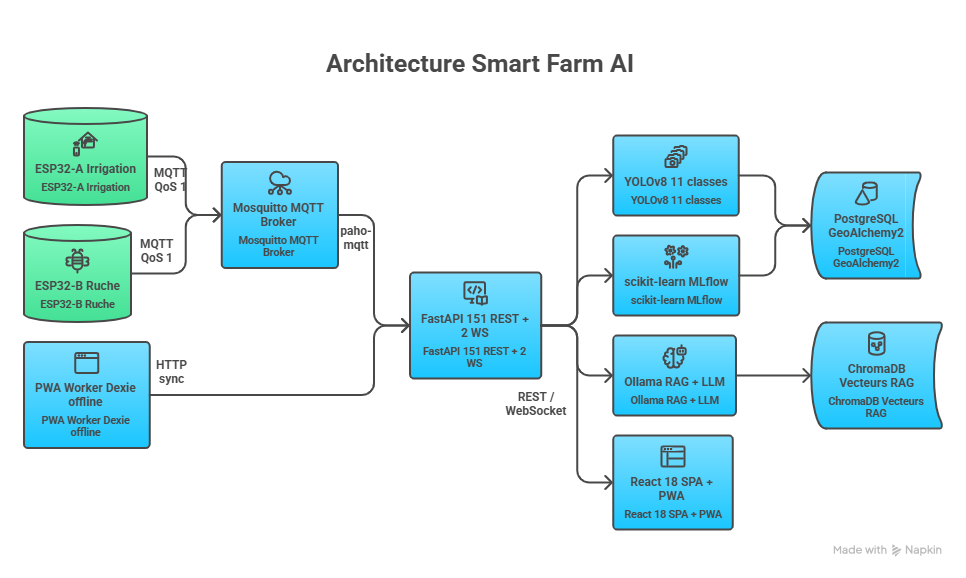
\includegraphics[width=\textwidth]{figures/architecture_smart_farm.png}
\caption[Architecture globale Smart Farm AI]{Vue globale de l'architecture Smart Farm AI }
\label{fig:archi_globale}
\end{figure}

\subsection{Vue d'ensemble de l'architecture}

L'architecture se décompose en quatre couches fonctionnelles superposées
(figure~\ref{fig:archi_4couches}), chacune ayant un périmètre de responsabilité
clairement délimité et communiquant avec ses voisines via des interfaces définies.

\begin{figure}[H]
\centering
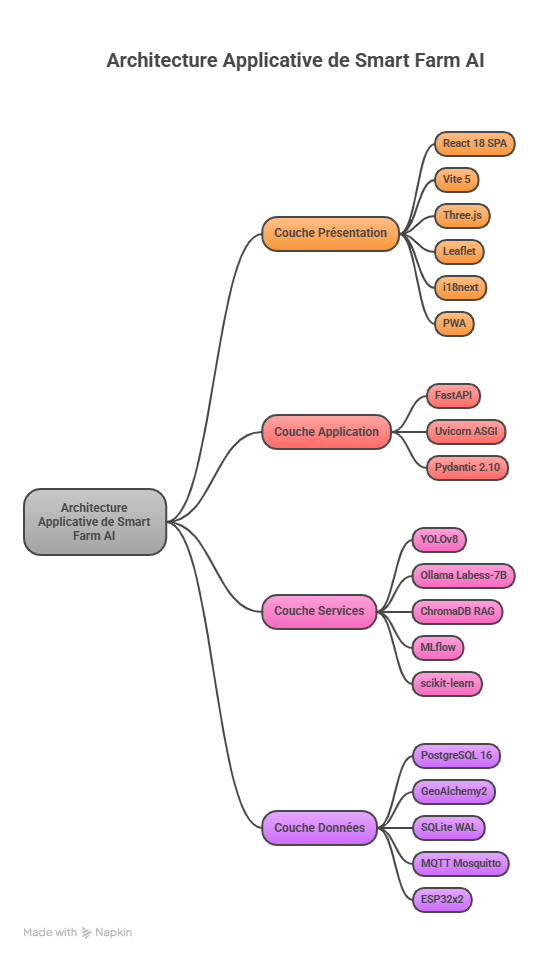
\includegraphics[width=0.92\textwidth]{figures/architecture_applicative_smart_farm.png}
\caption[Architecture applicative 4 couches]{Architecture applicative en 4 couches de Smart Farm AI.
Chaque couche communique avec la couche adjacente via une interface définie~.}
\label{fig:archi_4couches}
\end{figure}

\medskip

\begin{description}
  \item[Couche Présentation] Interface utilisateur construite avec React~18 (SPA)
        et compilée par Vite~5. Elle intègre Three.js pour la visualisation 3D
        des fermes (8 modèles GLB), Leaflet/MapLibre pour la cartographie GIS
        interactive, Recharts pour les graphiques de performance avicole et
        i18next pour l'internationalisation (FR/AR/EN, RTL). La Progressive Web App
        (PWA) utilise un Service Worker et Dexie IndexedDB pour fonctionner
        entièrement hors-ligne.
  \item[Couche Application] Backend REST et WebSocket développé avec FastAPI
        (Python~3.11) et servi par Uvicorn ASGI (2 workers). Elle expose
        151 endpoints répartis sur 22 fichiers de routes et 2 canaux WebSocket
        multi-tenant. La validation est assurée par Pydantic~2.10 ; la sécurité
        repose sur JWT HS256 et RBAC (rôles~: \texttt{owner}, \texttt{worker}).
  \item[Couche Services] Moteur IA regroupant YOLOv11 (détection 11 classes,
        mAP@50~$= 84.7\,\%$), Ollama + Labess-7B (LLM local Darija, GGUF Q4\_K\_M),
        ChromaDB (base vectorielle RAG, 312 chunks), scikit-learn (5 modèles avicoles)
        et MLflow (traçabilité MLOps). Tous les modèles fonctionnent localement~---~aucune
        dépendance à une API cloud externe.
  \item[Couche Données] Persistance sur PostgreSQL~16 avec extensions PostGIS
        (GeoAlchemy2, SRID~4326) pour les requêtes géographiques (ST\_DWithin) ;
        fallback SQLite WAL pour les déploiements légers (\texttt{LITE\_MODE}).
        La télémétrie IoT est acheminée via MQTT (broker Mosquitto, QoS~1)
        depuis deux nœuds ESP32.
\end{description}

\subsection{Composants de l'architecture}

La figure~\ref{fig:composants} détaille les interactions entre les composants
logiciels majeurs du système et leurs dépendances.

\begin{figure}[H]
\centering
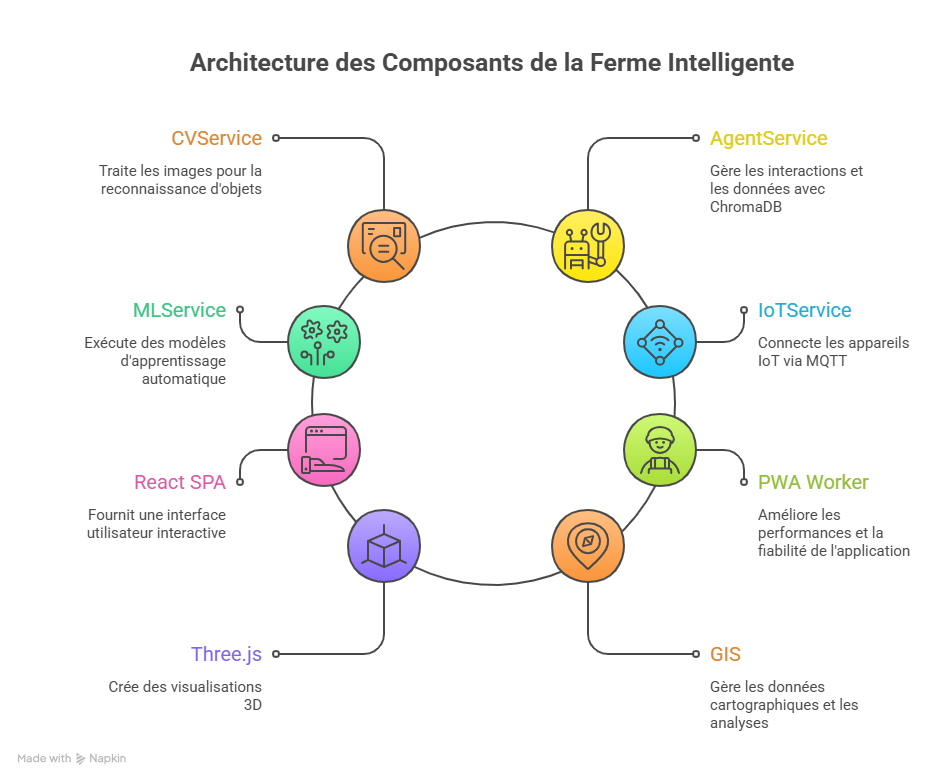
\includegraphics[width=\textwidth]{figures/architecture_composants_smart_farm.png}
\caption{Diagramme de composants Smart Farm AI }
\label{fig:composants}
\end{figure}

% ── 2.5 Besoins technologiques ──────────────────────────────
\section{Les besoins technologiques}

Le choix des technologies a été guidé par trois critères principaux~: la
\textit{souveraineté} (préférence systématique aux solutions open-source
auto-hébergées), la \textit{performance} sur infrastructure à ressources limitées
et la \textit{maturité} de l'écosystème garantissant la pérennité du projet.
Le tableau~\ref{tab:techno} présente l'ensemble des choix retenus et leur justification.

\begin{table}[H]
\centering
\caption[Besoins technologiques]{Besoins technologiques --- solutions choisies et justifications}
\label{tab:techno}
\resizebox{\textwidth}{!}{%
\begin{tabular}{llll}
\toprule
\textbf{Besoin} & \textbf{Solution choisie} & \textbf{Version} & \textbf{Justification} \\
\midrule
Interface SPA réactive, 3D, cartographie
  & React + Three.js + Leaflet/MapLibre
  & 18.2 / 0.183 / 1.9
  & Écosystème mature, WebGL natif, tiles open-source \\
\addlinespace
Bundler rapide, PWA offline
  & Vite + vite-plugin-pwa
  & 5.1 / 1.2
  & HMR $<50$\,ms, Service Worker, manifest configurables \\
\addlinespace
Cache requêtes, état global léger
  & TanStack Query + Zustand
  & 5.1 / 5.0
  & Invalidation automatique, store minimal sans Redux \\
\addlinespace
Persistance offline, sync différée
  & Dexie (IndexedDB)
  & 4.4
  & API Promise, schéma typé, migrations automatiques \\
\addlinespace
Internationalisation FR/AR/EN + RTL
  & i18next + react-i18next
  & 26.0 / 17.0
  & 400+ clés, détection langue auto, RTL CSS natif \\
\addlinespace
API REST asynchrone + WebSocket
  & FastAPI + Uvicorn ASGI
  & $\geq$0.100 / $\geq$0.24
  & ASGI natif, Pydantic~2 intégré, OpenAPI auto-généré \\
\addlinespace
Validation schémas, sérialisation
  & Pydantic
  & $\geq$2.10
  & Validation stricte, schémas auto pour OpenAPI \\
\addlinespace
Base de données relationnelle + géo
  & PostgreSQL~16 + GeoAlchemy2
  & 16 / $\geq$0.14
  & PostGIS ST\_DWithin, ACID complet, fallback SQLite WAL \\
\addlinespace
ORM + migrations
  & SQLAlchemy + Alembic
  & $\geq$2.0 / $\geq$1.12
  & Sessions async, 38 modèles, migrations versionnées \\
\addlinespace
Détection objets temps réel multi-classes
  & YOLOv11 (Ultralytics)
  & $\geq$8.1
  & anchor-free, mAP@50\,$=84.7\,\%$, CPU $\leq200$\,ms \\
\addlinespace
LLM local souverain Darija
  & Ollama + Labess-7B GGUF Q4\_K\_M
  & $\geq$0.1
  & Zéro dépendance cloud, fine-tune maghrébin, 4~GB RAM \\
\addlinespace
Base vectorielle RAG
  & ChromaDB + sentence-transformers
  & $\geq$0.4 / $\geq$2.5
  & k-NN persistant, multilingual-mpnet-base-v2 \\
\addlinespace
Modèles ML avicoles (5 types)
  & scikit-learn
  & $\geq$1.3
  & Régression poly., Random Forest, Isolation Forest \\
\addlinespace
Télémétrie IoT temps réel
  & MQTT Mosquitto + paho-mqtt + ESP32
  & 1.6 / WROOM-32
  & QoS~1, $\leq30$ oct./message, WLAN 802.11b/g/n \\
\addlinespace
Traçabilité MLOps
  & MLflow + DVC
  & $\geq$2.10 / $\geq$3.45
  & Reproductibilité totale, artifacts et datasets versionnés \\
\addlinespace
Sécurité, authentification multi-rôles
  & JWT HS256 + bcrypt + OTP WhatsApp
  & $\geq$3.3 / $\geq$4.0
  & Standard industrie, TTL 5\,min OTP, RBAC par endpoint \\
\addlinespace
Déploiement orchestré par conteneurs
  & Docker Compose + Nginx + Caddy (opt.)
  & 3.x / 1.25 / 2.x
  & Isolation services, HTTPS automatique Let's Encrypt \\
\bottomrule
\end{tabular}
}%
\end{table}

% ── 2.6 Planification CRISP-DM ──────────────────────────────
\section{Planification du projet}

La méthodologie CRISP-DM (\textit{Cross-Industry Standard Process for Data Mining})~%
\cite{wirth2000} a été adoptée comme cadre de planification du projet Smart Farm AI.
Ce modèle itératif en six phases est particulièrement adapté aux projets intégrant
des composantes de science des données et d'apprentissage automatique, car il structure
le cycle complet --- de la compréhension du domaine métier jusqu'au déploiement en
production --- en garantissant l'alignement permanent entre les besoins des
utilisateurs et les modèles développés.
Nous détaillons ci-après l'application des six phases CRISP-DM à notre projet.

\subsection*{Phase 1 --- Compréhension métier (\textit{Business Understanding})}

\textbf{Objectif.} Identifier les problèmes agronomiques que le système doit
résoudre et traduire les attentes des agriculteurs et des ouvriers en exigences
techniques mesurables.

\textbf{Activités menées.}
\begin{itemize}
  \item Analyse des processus métier agricoles (élevage multi-espèces,
        apiculture COLOSS, aviculture ERP, irrigation IoT) ;
  \item Identification de 12 besoins fonctionnels (BF-01\ldots BF-12) et
        6 critères non fonctionnels (performance, sécurité, disponibilité,
        scalabilité, i18n, portabilité) ;
  \item Modélisation des cas d'utilisation UML (2 acteurs, 8 sous-systèmes,
        21 cas d'utilisation avec relations \texttt{<<include>>} et
        \texttt{<<extend>>}).
\end{itemize}

\textbf{Livrable.} Cahier des charges fonctionnel, diagrammes UML de cas
d'utilisation (section~\ref{sec:uc}).

\subsection*{Phase 2 --- Compréhension des données (\textit{Data Understanding})}

\textbf{Objectif.} Inventorier et caractériser toutes les sources de données
nécessaires à l'entraînement et à l'évaluation des modèles.

\textbf{Sources identifiées.}
\begin{itemize}
  \item \textbf{Images YOLO} : 11 classes (bovins, ovins, caprins, lapins, poulets,
        abeilles, feux, maladies foliaires d'olive et d'agrumes) ---
        $\approx$\,8\,500 images annotées au format YOLO txt ;
  \item \textbf{Séries temporelles IoT} : mesures ESP32 toutes les 10--30\,s
        (humidité sol, pression hydraulique, température extérieure, poids ruche) ;
  \item \textbf{Corpus RAG} : guides AVFA, fiches vétérinaires tunisiennes,
        protocoles COLOSS BeeBook --- 47 documents PDF, 312 chunks indexés ;
  \item \textbf{Logs avicoles} : 500+ lots (FCR journalier, mortalité, ponte,
        consommation aliment) issus d'élevages du gouvernorat de Sfax.
\end{itemize}

\textbf{Livrable.} Rapport d'analyse exploratoire (distributions, corrélations,
premières détections d'outliers).

\subsection*{Phase 3 --- Préparation des données (\textit{Data Preparation})}

\textbf{Objectif.} Transformer les données brutes en entrées exploitables par
les modèles, en garantissant qualité et cohérence.

\textbf{Transformations appliquées.}
\begin{itemize}
  \item Augmentation images YOLO : rotation ($\pm15^{\circ}$), flip horizontal,
        mosaic 4-images, jitter HSV ; résolution normalisée $640\times640$ ;
  \item Normalisation Z-score des séries IoT ; interpolation linéaire pour
        les lacunes inférieures à $2\,\%$ ;
  \item Découpage des documents RAG en chunks de 512 tokens (chevauchement
        50 tokens), embeddings \texttt{paraphrase-multilingual-mpnet-base-v2} ;
  \item \texttt{TimeSeriesSplit} (5 plis) pour la validation croisée des
        modèles avicoles --- évite toute fuite temporelle.
\end{itemize}

\textbf{Livrable.} Pipelines DVC reproductibles (\texttt{dvc.yaml}),
datasets versionnés et traçables.

\subsection*{Phase 4 --- Modélisation (\textit{Modeling})}

\textbf{Objectif.} Entraîner et optimiser les modèles IA selon les tâches
identifiées lors des phases précédentes.

\begin{description}
  \item[YOLOv11] Fine-tuning sur 100 époques, batch~$= 16$,
        image~$= 640\times640$, optimiseur AdamW,
        \texttt{early\_stopping}~$= 10$.
  \item[Aviculture ML] Régression polynomiale deg.~2 (FCR), Random Forest
        ($n = 100$ arbres) pour la mortalité, ARIMA pour les séries de ponte.
  \item[RAG + LLM] Indexation ChromaDB avec top-$k = 5$, prompt
        espèce-spécifique, modèle Labess-7B quantifié Q4\_K\_M via Ollama.
  \item[Anomalies IoT] Isolation Forest (contamination~$= 0.05$)~%
        \cite{liu2008isolation} sur les séries temporelles de capteurs.
\end{description}

\textbf{Livrable.} Modèles entraînés versionnés (MLflow),
hyperparamètres documentés (annexe~D).

\subsection*{Phase 5 --- Évaluation (\textit{Evaluation})}

\textbf{Objectif.} Valider statistiquement que les modèles satisfont les
critères de qualité définis en phase~1 et identifier les menaces à la validité.

\textbf{Métriques et résultats.}
\begin{itemize}
  \item YOLOv11 : mAP@50~$= 84.7\,\%\ \pm 0.45\,\%$ (5-fold CV)
  \item FCR polynomial : $R^2 = 0.891 \pm 0.024$ (TimeSeriesSplit 5 plis)
  \item RAG Darija : BLEU-4~$= 0.68$, ROUGE-L~$= 0.72$,
        Cohen's~$\kappa = 0.76$~\cite{cohen1960,landis1977}
  \item Latence API : p50~$= 67$\,ms, p95~$= 143$\,ms
        (50 utilisateurs simultanés)
\end{itemize}

Les intervalles de confiance à 95\,\% ont été calculés par \textit{bootstrap}
($B = 1\,000$ itérations) sur chaque ensemble de test indépendant.

\textbf{Livrable.} Rapport d'évaluation avec IC~95\,\%, section
\textit{Menaces à la validité} (validité interne, externe, de construct).

\subsection*{Phase 6 --- Déploiement (\textit{Deployment})}

\textbf{Objectif.} Rendre le système opérationnel en production sur
l'infrastructure de la ferme avec une disponibilité maximale et une
indépendance totale vis-à-vis des services cloud.

\textbf{Architecture de déploiement.}
\begin{itemize}
  \item Docker Compose : PostgreSQL~16 + FastAPI Uvicorn (2 workers)
        + React/Nginx (port~80) ;
  \item Caddy optionnel pour HTTPS automatique via Let's Encrypt ;
  \item PWA installable : Service Worker + IndexedDB Dexie pour les
        ouvriers terrain sans connexion permanente ;
  \item Fallback LLM en cascade~:
        Ollama (local) $\rightarrow$ Groq API (cloud) $\rightarrow$
        réponse statique Darija.
\end{itemize}

\textbf{Livrable.} Guide de déploiement (\texttt{SMART\_FARM\_RUN.md}),
image Docker versionée, scripts de \textit{seed} de données initiales.

\begin{figure}[H]
\centering
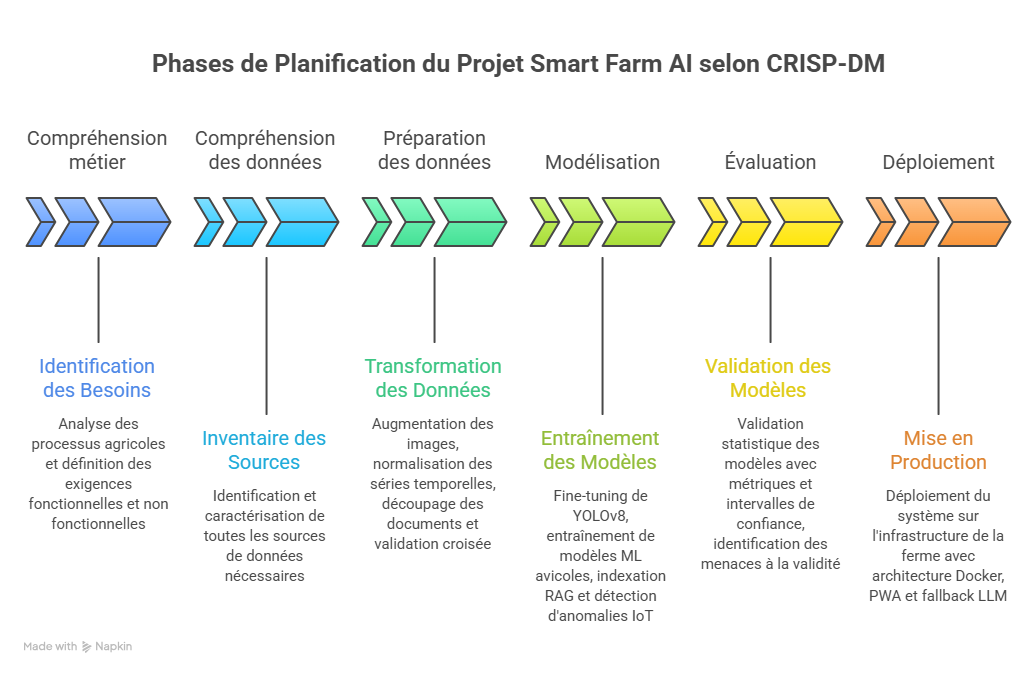
\includegraphics[width=\textwidth]{figures/phases_planification_smart_farm_crispdm.png}
\caption[Planification CRISP-DM]{Phases de Planification du Projet Smart Farm AI selon CRISP-DM}
\label{fig:phases_planification_smart_farm_crispdm}
\end{figure}

% ── 2.7 Conclusion ──────────────────────────────────────────
\section*{Conclusion}
\addcontentsline{toc}{section}{Conclusion}

Ce chapitre a posé les fondements analytiques et conceptuels du projet Smart Farm AI.
L'identification des besoins a formalisé 12 modules fonctionnels et 6 critères
non fonctionnels couvrant l'intégralité de la chaîne de valeur agricole.
Les diagrammes de cas d'utilisation UML ont illustré les interactions entre les
deux acteurs principaux (Propriétaire et Ouvrier PWA) et les huit sous-systèmes.
La revue des six travaux récents a permis de positionner notre contribution par
rapport à l'état de l'art~: notre système intègre IoT multi-nœuds, détection
YOLO multi-classes, prédiction avicole et RAG souverain en Darija tunisienne,
adressant ainsi les lacunes structurelles identifiées (absence d'évaluation en
Darija, dépendance cloud, fragmentation par espèce, insuffisance de rigueur
statistique).

L'architecture en quatre couches --- Présentation, Application, Services et Données ---
assure la séparation des responsabilités et la maintenabilité du système.
Le choix exclusif de technologies open-source (FastAPI, YOLOv11, Ollama,
ChromaDB, PostgreSQL) garantit la souveraineté technologique et la
reproductibilité scientifique. Enfin, la planification selon CRISP-DM structure
le développement en six phases itératives, de la compréhension métier jusqu'au
déploiement en production.

Le chapitre suivant présente la modélisation détaillée du système et l'évaluation
quantitative des performances des modèles IA développés.

% ============================================================
%  CHAPITRE 3 : MODÉLISATION ET ÉVALUATION DES PERFORMANCES
% ============================================================